\chapter{嘉当子代数与正则元}

本章中，k 表示一个（交换）域。所谓“向量空间”，我们指“k 上的向量空间”；“李代数”等术语亦按同样方式理解。所有李代数均假定为有限维。

\section{线性表示的准素分解}

\subsection{自同态族的分解}

设 V 是一个向量空间，S 是一个集合，r 是从 S 到 End(V) 中的一个映射。用 P 表示从 S 到 k 的映射所成的集合。若 \(\lambda \in P\) ，则用 \(\mathrm{V}_{\lambda}(\mathrm{S})\) （相应地，\(\mathrm{V}^{\lambda}(\mathrm{S})\) ）表示满足下列条件的 \(v \in V\) 所成的集合：对所有 \(s \in S\) ，\(r(s)v = \lambda(s)v\) （相应地，\((r(s) - \lambda(s))^{n}v = 0\) 对充分大的 n 成立）。集合 \(\mathrm{V}_{\lambda}(\mathrm{S})\) 与 \(\mathrm{V}^{\lambda}(\mathrm{S})\) 都是 V 的向量子空间，且 \(\mathrm{V}_{\lambda}(\mathrm{S}) \subset \mathrm{V}^{\lambda}(\mathrm{S})\) 。我们称 \(\mathrm{V}_{\lambda}(\mathrm{S})\) 为 V 相对于 \(\lambda\) （以及 r）的特征子空间，称 \(\mathrm{V}^{\lambda}(\mathrm{S})\) 为 V 相对于 \(\lambda\) （以及 r）的准素子空间，并称 \(\mathrm{V}^{0}(\mathrm{S})\) 为 V 的（相对于 r 的）幂零空间。我们称 \(\lambda\) 是 S 在 V 中的一个权，如果 \(\mathrm{V}^{\lambda}(\mathrm{S}) \neq 0\) 。

特别地，若 S 只含单个元素 s，则 P 可与 k 等同；这时我们用记号 \(\mathrm{V}_{\lambda(s)}(s)\) 与 \(\mathrm{V}^{\lambda(s)}(s)\) ，或 \(\mathrm{V}_{\lambda(s)}(r(s))\) 与 \(\mathrm{V}^{\lambda(s)}(r(s))\) ，来代替 \(\mathrm{V}_{\lambda}(\{s\})\) 、\(\mathrm{V}^{\lambda}(\{s\})\) ；我们说 \(r(s)\) 的特征子空间、准素子空间与幂零空间；\(\mathrm{V}_{\lambda(s)}(s)\) 中的元素 v 称为 \(r(s)\) 的特征向量，且当 \(v \neq 0\) 时，\(\lambda(s)\) 称为相应的特征值（参看~代数，第七章，§5）。

对所有 \(\lambda\in P\) ，下列关系式是直接的：

\[
V ^ {\lambda} (S) = \bigcap_ {s \in S} V ^ {\lambda (s)} (s),\tag{1}
\]

\[
V _ {\lambda} (S) = \bigcap_ {s \in S} V _ {\lambda (s)} (s).\tag{2}
\]

设 \(k'\) 是 \(k\) 的一个扩张。从 \(\operatorname{End}(V)\) 到 \(\operatorname{End}(V \otimes_k k')\) 的典则映射与 \(r\) 复合，给出一个映射 \(r' : S \to \operatorname{End}(V \otimes_k k')\) 。类似地，任何映射 \(\lambda\) （从 S 到 \(k\) ）都典则地定义一个映射，仍记作 \(\lambda\) （从 S 到 \(k'\) ）。在这些记号下，我们有以下命题：

命题 1. 对所有 \(\lambda \in \mathrm{P}\) ，

\[
(\mathrm{V} \otimes_ {k} k ^ {\prime}) ^ {\lambda} (\mathrm{S}) = \mathrm{V} ^ {\lambda} (\mathrm{S}) \otimes_ {k} k ^ {\prime} \text {and} (\mathrm{V} \otimes_ {k} k ^ {\prime}) _ {\lambda} (\mathrm{S}) = \mathrm{V} _ {\lambda} (\mathrm{S}) \otimes_ {k} k ^ {\prime}.
\]

设 \((a_{i})\) 是 k-向量空间 \(k'\) 的一个基。若 \(v \in V \otimes_{k} k'\) ，则 v 可唯一地表示为 \(\sum v_{i} \otimes a_{i}\) 的形式，其中 \((v_{i})\) 是 V 中元素的一个有限支集族。对所有 \(s \in S\) ，

\[
(r ^ {\prime} (s) - \lambda (s)) ^ {n} (v) = \sum (r (s) - \lambda (s)) ^ {n} v _ {i} \otimes a _ {i}.
\]

由此得出

\[
v \in (\mathrm{V} \otimes_ {k} k ^ {\prime}) ^ {\lambda} (\mathrm{S}) \Longleftrightarrow v _ {i} \in \mathrm{V} ^ {\lambda} (\mathrm{S}) \text { for   all } i,
\]

\[
v \in (\mathrm{V} \otimes_ {k} k ^ {\prime}) _ {\lambda} (\mathrm{S}) \Longleftrightarrow v _ {i} \in \mathrm{V} _ {\lambda} (\mathrm{S}) \text { for   all } i,
\]

这就蕴含该命题。

命题 2. 设 \(\mathrm{V}, \mathrm{V}'\) 、\(\mathrm{W}\) 为向量空间。设 \(r: \mathrm{S} \to \operatorname{End}(\mathrm{V})\) 、\(r': \mathrm{S} \to \operatorname{End}(\mathrm{V}')\) 与 \(q: \mathrm{S} \to \operatorname{End}(\mathrm{W})\) 为映射。

\begin{enumerate}
\def\labelenumi{(\roman{enumi})}
\item
  设 \(f: \mathrm{V} \to \mathrm{W}\) 是线性映射，使得 \(q(s)f(v) = f(r(s)v)\) 对 \(s \in \mathrm{S}\) 与 \(v \in \mathrm{V}\) 成立。那么，对所有 \(\lambda \in \mathrm{P}\) ，\(f\) 把 \(\mathrm{V}^{\lambda}(\mathrm{S})\) （相应地，\(\mathrm{V}_{\lambda}(\mathrm{S})\) ）映入 \(W^{\lambda}(\mathrm{S})\) （相应地，\(W_{\lambda}(\mathrm{S})\) ）。
\item
  设 \(\mathrm{B}:\mathrm{V}\times \mathrm{V}'\to \mathrm{W}\) 是双线性映射，使得
\end{enumerate}

\[
q (s) \mathrm{B} (v, v ^ {\prime}) = \mathrm{B} (r (s) v, v ^ {\prime}) + \mathrm{B} (v, r ^ {\prime} (s) v ^ {\prime})
\]

其中 \(s \in \mathrm{S}\) ，\(v \in \mathrm{V}\) ，\(v' \in \mathrm{V}'\) 。那么，对所有 \(\lambda, \mu \in \mathrm{P}\) ，B 把 \(V^{\lambda}(\mathrm{S}) \times \mathrm{V}'^{\mu}(\mathrm{S})\) （相应地，\(\mathrm{V}_{\lambda}(\mathrm{S}) \times \mathrm{V}_{\mu}'(\mathrm{S})\) ）映入 \(W^{\lambda + \mu}(\mathrm{S})\) （相应地，\(W_{\lambda + \mu}(\mathrm{S})\) ）。

\begin{enumerate}
\def\labelenumi{(\roman{enumi})}
\setcounter{enumi}{2}
\tightlist
\item
  设 \(B: V \times V' \to W\) 是双线性映射，使得
\end{enumerate}

\[
q (s) \mathrm{B} (v, v ^ {\prime}) = \mathrm{B} (r (s) v, r ^ {\prime} (s) v ^ {\prime})
\]

其中 \(s \in S\) ，\(v \in V\) ，\(v' \in V'\) 。那么，对所有 \(\lambda, \mu \in P\) ，B 把 \(V^{\lambda}(S) \times V'^{\mu}(S)\) （相应地，\(V_{\lambda}(S) \times V'_{\mu}(S)\) ）映入 \(W^{\lambda\mu}(S)\) （相应地，\(W_{\lambda\mu}(S)\) ）。

在情形 (i) 中，\((q(s) - \lambda(s))^n f(v) = f((r(s) - \lambda(s))^n v)\) 对 \(s \in S\) 与 \(v \in V\) 成立，由此即得结论。在情形 (ii) 中，

\[
(q (s) - \lambda (s) - \mu (s)) \mathrm{B} (v, v ^ {\prime}) = \mathrm{B} ((r (s) - \lambda (s)) v, v ^ {\prime}) + \mathrm{B} (v, (r ^ {\prime} (s) - \mu (s)) v ^ {\prime})
\]

其中 \(s \in S\) ，\(v \in V\) ，\(v' \in V'\) ，从而对 n 用归纳法得

\[
(q (s) - \lambda (s) - \mu (s)) ^ {n} \mathrm{B} (v, v ^ {\prime}) = \sum_ {i + j = n} \binom {n} {i} \mathrm{B} ((r (s) - \lambda (s)) ^ {i} v, (r ^ {\prime} (s) - \mu (s)) ^ {j} v ^ {\prime}).
\]

(ii) 中的断言立即可得。在情形 (iii) 中，

\[
(q (s) - \lambda (s) \mu (s)) \mathrm{B} (v, v ^ {\prime}) = \mathrm{B} ((r (s) - \lambda (s)) v, r ^ {\prime} (s) v ^ {\prime}) + \mathrm{B} (\lambda (s) v, (r ^ {\prime} (s) - \mu (s)) v ^ {\prime})
\]

其中 \(s \in S\) ，\(v \in V\) ，\(v' \in V'\) ，从而对 n 用归纳法得

\[
\begin{array}{l} (q (s) - \lambda (s) \mu (s)) ^ {n} \mathrm{B} (v, v ^ {\prime}) \\ = \sum_ {i + j = n} \binom {n} {i} \mathrm{B} (\lambda (s) ^ {j} (r (s) - \lambda (s)) ^ {i} v, r ^ {\prime} (s) ^ {i} (r ^ {\prime} (s) - \mu (s)) ^ {j} v ^ {\prime}). \end{array}
\]

(iii) 中的断言立即可得。

命题 3. 和 \(\sum_{\lambda \in \mathrm{P}}\mathrm{V}^{\lambda}(\mathrm{S})\) 是直和。和 \(\sum_{\lambda \in \mathrm{P}}\mathrm{V}_{\lambda}(\mathrm{S})\) 是直和。

第二个断言是第一个断言的推论；因此只需证明后者。我们区分几种情形。

\begin{enumerate}
\def\labelenumi{\alph{enumi})}
\item
  S 为空集。断言是平凡的。
\item
  S 只含单个元素 s。设 \(\lambda_{0}, \lambda_{1}, \ldots, \lambda_{n}\) 是 k 中互异的元素。对 \(i = 0, 1, \ldots, n\) ，设 \(v_{i} \in V^{\lambda_{i}}(s)\) 且假定 \(v_{0} = v_{1} + \cdots + v_{n}\) 。只需证明 \(v_{0} = 0\) 。对 \(i = 0, \ldots, n\) ，存在整数 \(q_{i} > 0\) 使得 \((r(s) - \lambda_{i})^{q_{i}} v_{i} = 0\) 。考虑多项式 \(\mathrm{P}(\mathrm{X}) = \prod_{i \geq 1} (\mathrm{X} - \lambda_{i})^{q_{i}}\) 与 \(\mathrm{Q}(\mathrm{X}) = (\mathrm{X} - \lambda_{0})^{q_{0}}\) 。我们有 \(\mathrm{Q}(r(s)) v_{0} = 0\) ，以及 \(\mathrm{P}(r(s)) v_{0} = \sum_{i=1}^{n} \mathrm{P}(r(s)) v_{i} = 0\) 。由于 P 与 Q 互素，Bezout 恒等式表明 \(v_{i} = 0\) 。
\end{enumerate}

\[
v _ {0} = 0
\]

\begin{enumerate}
\def\labelenumi{\alph{enumi})}
\setcounter{enumi}{2}
\item
  S 有限且非空。我们对 S 的基数作归纳。设 \(s \in \mathrm{S}\) ，并设 \(\mathrm{S}' = \mathrm{S} - \{s\}\) 。设 \((v_{\lambda})_{\lambda \in \mathrm{P}}\) 是 V 中元素的一个有限支集族，满足 \(\sum_{\lambda \in \mathrm{P}} v_{\lambda} = 0\) 且 \(v_{\lambda} \in \mathrm{V}^{\lambda}(\mathrm{S})\) 。取 \(\lambda_0 \in \mathrm{P}\) 。设 \(\mathrm{P}'\) 是 \(\lambda \in \mathrm{P}\) 中使 \(\lambda |\mathrm{S}' = \lambda_0|\mathrm{S}'\) 的元素所成的集合。对 \(\mathrm{S}'\) 应用归纳假设，得 \(\sum_{\lambda \in \mathrm{P}'} v_{\lambda} = 0\) 。若 \(\lambda, \mu\) 是 \(\mathrm{P}'\) 中互异的元素，则 \(\lambda(s) \neq \mu(s)\) 。由于和 \(\sum_{\alpha \in k} \mathrm{V}^{\alpha}(s)\) 依 \(b\) ) 是直和，且 \(v_{\lambda} \in \mathrm{V}^{\lambda(s)}(s)\) ，故 \(v_{\lambda} = 0\) 对所有 \(\lambda \in \mathrm{P}'\) 成立，特别地 \(v_{\lambda_0} = 0\) ，此即所要证明的。
\item
  一般情形。设 \((v_{\lambda})_{\lambda\in\mathrm{P}}\) 是 V 中元素的一个有限支集族，满足 \(\sum_{\lambda\in\mathrm{P}} v_{\lambda}=0\) 且 \(v_{\lambda}\in\mathrm{V}^{\lambda}(\mathrm{S})\) 。设 \(P'\) 是 \(\lambda\in P\) 中使 \(v_{\lambda}\neq0\) 的元素所成的有限集合，并设 \(S'\) 是 S 的一个有限子集，使得条件 \(\lambda\in P'\) 、\(\mu\in P'\) 、\(\lambda|S'= \mu|S'\) 蕴含 \(\lambda=\mu\) 。我们有 \(v_{\lambda}\in\mathrm{V}^{\lambda|S'}(S')\) ；应用 c)，即知 \(v_{\lambda}=0\) 对 \(\lambda\in P'\) 成立，证毕。
\end{enumerate}

回顾一下，若 \(x \in \operatorname{End}(\mathrm{V})\) ，我们用 ad \(x\) 表示映射 \(y \mapsto xy - yx = [x, y]\) ，它从 \(\operatorname{End}(\mathrm{V})\) 到其自身。

引理 1. 设 \(x, y \in \operatorname{End}(\mathbf{V})\) 。

\begin{enumerate}
\def\labelenumi{(\roman{enumi})}
\item
  假定 \(\mathrm{V}\) 是有限维的。那么 \(x\) 可三角化当且仅当 \(\mathrm{V} = \sum_{a\in k}\mathrm{V}^a (x)\) 。
\item
  若存在整数 \(n\) 使 \((\mathrm{ad}x)^n y = 0\) ，则每个 \(\mathrm{V}^a(x)\) 在 \(y\) 下稳定。
\item
  假定 \(\mathrm{V}\) 是有限维的。若 \(\mathrm{V} = \sum_{a \in k} \mathrm{V}^a(x)\) 且每个 \(\mathrm{V}^a(x)\) 在 \(y\) 下稳定，则存在整数 \(n\) 使 \((\operatorname{ad} x)^n y = 0\) 。
\end{enumerate}

(i) 由代数，第七章，§5，第 2 节，命题 3 得出。

设 \(\mathrm{E} = \operatorname{End}(\mathrm{V})\) 。设 B 是双线性映射 \((u, v) \mapsto u(v)\) ，从 \(\mathrm{E} \times \mathrm{V}\) 到 V。由 ad \(x\) 的定义，

\[
x (\mathrm{B} (u, v)) = B (u, x (v)) + \mathrm{B} ((\operatorname{ad} x) (u), v)
\]

其中 \(x \in \mathrm{E}\) ，\(u \in \mathrm{E}\) ，\(v \in \mathrm{V}\) 。让 \(x\) 作用在 \(\mathrm{E}\) 上，作用经由 \(\operatorname{ad} x\) 。由命题 2 (ii)，\(\mathrm{B}(\mathrm{E}^0(x), \mathrm{V}^a(x)) \subset \mathrm{V}^a(x)\) 对所有 \(a \in k\) 成立。若 \((\operatorname{ad} x)^n y = 0\) ，则 \(y \in \mathrm{E}^0(x)\) ，故 \(y(\mathrm{V}^a(x)) \subset \mathrm{V}^a(x)\) ，这就证明了 (ii)。

为证明 (iii)，可把 V 换成 \(V^{a}(x)\) ，并把 x（相应地，y）换成它在 \(V^{a}(x)\) 上的限制。把 x 换成 x - a 后，可假定 x 是幂零的。于是 \((\operatorname{ad} x)^{2\dim V-1} = 0\) （第一章，§4，第 2 节），这就证明了 (iii)。

注. 上面的论证表明，若 V 是有限维的且存在整数 n 使 \((\operatorname{ad} x)^{n}y = 0\) ，则 \((\operatorname{ad} x)^{2\dim V-1}y = 0\) 。

以后我们说映射 \(r : S \to \text{End}(V)\) 满足条件 (AC)（“拟交换”）是指：

(AC) 对 S 的每一对元素 \((s, s')\) ，存在整数 \(n\) 使得

\[
(\operatorname{ad} r (s)) ^ {n} r \left(s ^ {\prime}\right) = 0.
\]

定理 1. 假定 V 是有限维的。下列条件等价：

\begin{enumerate}
\def\labelenumi{(\roman{enumi})}
\item
  条件 (AC) 满足，且对所有 \(s \in \mathrm{S}\) ，\(r(s)\) 可三角化。
\item
  对所有 \(\lambda \in \mathrm{P}\) ，\(\mathrm{V}^{\lambda}(\mathrm{S})\) 在 \(r(\mathrm{S})\) 下稳定，且 \(\mathrm{V} = \sum_{\lambda \in \mathrm{P}} \mathrm{V}^{\lambda}(\mathrm{S})\) 。
\end{enumerate}

若 \(V = \sum_{\lambda \in P} V^{\lambda}(S)\) ，则 \(V = \sum_{a \in k} V^{a}(s)\) 对所有 \(s \in S\) 成立，于是由引理 1 可知 (ii) 蕴含 (i)。假定条件 (i) 满足。引理 1 与公式 (1) 表明每个 \(V^{\lambda}(S)\) 在 \(r(S)\) 下稳定。剩下要证 \(V = \sum_{\lambda \in P} V^{\lambda}(S)\) 。我们对 dim V 作归纳。我们区分两种情形。

\(a)\) 对所有 \(s \in \mathrm{S}\) ，\(r(s)\) 只有一个特征值 \(\lambda(s)\) 。于是 \(\mathrm{V} = \mathrm{V}^{\lambda}(\mathrm{S})\) 。

\begin{enumerate}
\def\labelenumi{\alph{enumi})}
\setcounter{enumi}{1}
\tightlist
\item
  存在 \(s \in S\) 使 \(r(s)\) 至少有两个互异的特征值。于是 V 是诸 \(\mathrm{V}^{a}(s)\) （\(a \in k\) ）的直和，且对所有 a 有 \(\dim \mathrm{V}^{a}(s) < \dim \mathrm{V}\) 。每个 \(\mathrm{V}^{a}(s)\) 在 \(r(\mathrm{S})\) 下稳定，只需应用归纳假设即可。
\end{enumerate}

推论 1. 假定 V 是有限维的且条件 (AC) 满足。设 \(k'\) 是 \(k\) 的一个扩张。假定对所有 \(s \in S\) ，\(r(s) \otimes 1\) 作为 \(V \otimes_k k'\) 的自同态可三角化。设 \(P'\) 是从 \(S\) 到 \(k'\) 的映射所成的集合。那么 \(V \otimes_k k' = \sum_{\lambda' \in P'} (V \otimes_k k')^{\lambda'}(S)\) 。

设 \(r': S \to \operatorname{End}(V \otimes_k k')\) 是由 \(r\) 定义的映射。若 \(s_1, s_2 \in S\) ，则存在整数 \(n\) 使 \((\operatorname{ad} r(s_1))^n r(s_2) = 0\) ，从而 \((\operatorname{ad} r'(s_1))^n r'(s_2) = 0\) 。现在只需应用定理 1。

推论 2. 假定 V 是有限维的且条件 (AC) 满足。用 \(\mathrm{V}^{+}(\mathrm{S})\) 表示向量子空间 \(\sum_{s\in \mathrm{S}}\left(\bigcap_{i\geq 1}r(s)^{i}\mathrm{V}\right)\) 。那么：

\begin{enumerate}
\def\labelenumi{(\roman{enumi})}
\item
  \(\mathrm{V}^0 (\mathrm{S})\) 与 \(\mathrm{V^{+}(S)}\) 在 \(r(\mathrm{S})\) 下稳定；
\item
  \(\mathrm{V} = \mathrm{V}^{0}(\mathrm{S}) \oplus \mathrm{V}^{+}(\mathrm{S});\)
\item
  V 的每个在 \(r(\mathrm{S})\) 下稳定且满足 \(\mathrm{W}^0 (\mathrm{S}) = 0\) 的向量子空间 W 都包含于 \(\mathrm{V}^{+}(\mathrm{S})\) ；
\item
  \(\sum_{s\in S}r(s)\mathrm{V}^{+}(\mathrm{S}) = \mathrm{V}^{+}(\mathrm{S}).\)
\end{enumerate}

此外，\(V^{+}(S)\) 是 V 中唯一具有性质 (i) 与 (ii) 的向量子空间。对 k 的任何扩张 \(k'\) ，有 \((\mathrm{V} \otimes_{k} k')^{+}(\mathrm{S}) = \mathrm{V}^{+}(\mathrm{S}) \otimes_{k} k'\) 。

最后一个断言是直接的。于是，顾及命题 1，在证明其余断言时可假定 k 是代数闭的。由定理 1，\(V = \sum_{\lambda \in P} V^{\lambda}(S)\) ，且诸 \(V^{\lambda}(S)\) 在 \(r(S)\) 下稳定。若 \(s \in S\) ，则 \(r(s)|V^{\lambda}(S)\) 的特征多项式为 \((X - \lambda(s))^{\dim V^{\lambda}(S)}\) ；由此得出，\(\bigcap_{i \geq 1} r(s)^{i} V^{\lambda}(s)\) 为零，如果 \(\lambda(s) = 0\) ；而等于 \(V^{\lambda}(S)\) ，如果 \(\lambda(s) \neq 0\) ；因此，

\[
\mathrm{V} ^ {+} (\mathrm{S}) = \sum_ {\lambda \in \mathrm{P}, \lambda \neq 0} \mathrm{V} ^ {\lambda} (\mathrm{S}),\tag{3}
\]

这就证明了 (i)、(ii) 与 (iv)。若 W 是 V 的一个在 \(r(S)\) 下稳定的向量子空间，则 \(W = \sum_{\lambda \in P} W^{\lambda}(S)\) 且 \(W^{\lambda}(S) = W \cap V^{\lambda}(S)\) 。若 \(W^{0}(S) = 0\) ，则可见 \(W \subset V^{+}(S)\) ，这就证明了 (iii)。

设 \(V'\) 是 \(V\) 的一个在 \(r(S)\) 下稳定且满足 \(V' \cap V^0(S) = 0\) 的向量子空间。于是 \(V'^0(S) = 0\) ，故由 (iii) 得 \(V' \subset V^+(S)\) 。若此外还有 \(V = V^0(S) + V'\) ，则可见 \(V' = V^+(S)\) 。证毕。

我们有时把 \((\mathrm{V}^{0}(\mathrm{S}),\mathrm{V}^{+}(\mathrm{S}))\) 称为 V 的、或映射 \(r:S\to\operatorname{End}(\mathrm{V})\) 的 Fitting 分解。若 S 只含单个元素 s，我们用 \(\mathrm{V}^{+}(s)\) 或 \(\mathrm{V}^{+}(r(s))\) 代替 \(\mathrm{V}^{+}(\{s\})\) 。我们有 \(\mathrm{V}=\mathrm{V}^{0}(s)\oplus\mathrm{V}^{+}(s)\) ，\(\mathrm{V}^{0}(s)\) 与 \(\mathrm{V}^{+}(s)\) 在 \(r(s)\) 下稳定，\(r(s)|\mathrm{V}^{0}(s)\) 幂零而 \(r(s)|\mathrm{V}^{+}(s)\) 双射。

推论 3. 设 V 与 V' 是有限维向量空间，\(r: S \to \text{End}(V)\) 与 \(r': S \to \text{End}(V')\) 是满足条件 (AC) 的映射。设 \(f: V \to V'\) 是满射线性映射，使得 \(f(r(s)v) = r'(s)f(v)\) 对 \(s \in S\) 与 \(v \in V\) 成立。那么 \(f(V^{\lambda}(S)) = V'^{\lambda}(S)\) 对所有 \(\lambda \in P\) 成立。

鉴于命题 1，可化归到 \(k\) 是代数闭域的情形。由定理 1，我们有 \(\mathrm{V} = \bigoplus_{\lambda \in \mathrm{P}} \mathrm{V}^{\lambda}(\mathrm{S})\) ，\(\mathrm{V}' = \bigoplus_{\lambda \in \mathrm{P}} \mathrm{V}'^{\lambda}(\mathrm{S})\) ，以及 \(\mathrm{V}' = f(\mathrm{V}) = \sum_{\lambda \in \mathrm{P}} f(\mathrm{V}^{\lambda}(\mathrm{S}))\) 。最后，由命题 2 (i) 有 \(f(\mathrm{V}^{\lambda}(\mathrm{S})) \subset \mathrm{V}'^{\lambda}(\mathrm{S})\) ，由此即得推论。

命题 4. 假定 \(k\) 是完全域。设 \(V\) 是有限维向量空间，\(u\) 是 \(\operatorname{End}(V)\) 中的一个元素，\(u_s, u_n\) 是 \(u\) 的半单分量与幂零分量（代数，第七章，§5，第 8 节）。

\begin{enumerate}
\def\labelenumi{(\roman{enumi})}
\item
  对所有 \(\lambda \in k\) ，\(V^{\lambda}(u) = V^{\lambda}(u_s) = V_{\lambda}(u_s)\) 。
\item
  若 \(\mathrm{V}\) 具有一个代数结构且 \(u\) 是 \(\mathrm{V}\) 的导子，则 \(u_{s}\) 与 \(u_{n}\) 是 \(\mathrm{V}\) 的导子。
\item
  若 \(\mathrm{V}\) 具有一个代数结构且 \(u\) 是 \(\mathrm{V}\) 的自同构，则 \(u_{s}\) 与 \(1 + u_{s}^{-1}u_{n}\) 是 \(\mathrm{V}\) 的自同构。
\end{enumerate}

鉴于命题 1，可假定 \(k\) 是代数闭的，于是

\[
\mathrm{V} = \sum_ {\lambda \in k} \mathrm{V} ^ {\lambda} (u).
\]

\(u|V^{\lambda}(u)\) 的半单分量是比率为 \(\lambda\) 的、\(V^{\lambda}(u)\) 中的位似。这就证明了 (i)。

以下假定 \(\mathrm{V}\) 具有一个代数结构。设 \(x \in \mathrm{V}^{\lambda}(u)\) ，\(y \in \mathrm{V}^{\mu}(u)\) 。

若 \(u\) 是 \(\mathrm{V}\) 的导子，则 \(xy \in \mathrm{V}^{\lambda + \mu}(u)\) （命题 2 (ii)），于是

\[
u _ {s} (x y) = (\lambda + \mu) (x y) = (\lambda x) y + x (\mu y) = (u _ {s} x) y + x (u _ {s} y).
\]

这证明 \(u_{s}\) 是 V 的导子。于是 \(u_{n} = u - u_{s}\) 是 V 的导子。

若 u 是 V 的自同构，则 \(\operatorname{Ker}(u_{s}) = \mathrm{V}^{0}(u) = 0\) ，故 \(u_{s}\) 双射。另一方面，\(xy \in \mathrm{V}^{\lambda\mu}(u)\) （命题 2 (iii)），于是

\[
u _ {s} (x y) = (\lambda \mu) (x y) = (\lambda x) (\mu y) = u _ {s} (x). u _ {s} (y).
\]

这证明 \(u_{s}\) 是 V 的自同构；而如下元素也是自同构：

\[
1 + u _ {s} ^ {- 1} u _ {n} = u _ {s} ^ {- 1} u.
\]

\subsection{线性自同态族的情形}

现在假定 S 具有一个向量空间结构，映射 \(r : S \to \text{End}(V)\) 是线性的，且 V 与 S 都是有限维的。

命题 5. 假定条件 (AC) 满足，并设 \(\lambda : S \to k\) 使 \(V^{\lambda}(S) \neq 0\) 。若 \(k\) 的特征为 0，则映射 \(\lambda\) 是线性的。若 \(k\) 的特征为 \(p \neq 0\) ，则存在 \(q\) （\(p\) 的一个幂）整除 \(\dim V^{\lambda}(S)\) ，以及一个齐次多项式函数 \(P : S \to k\) ，次数为 \(q\) ，使得 \(\lambda(s)^{q} = P(s)\) 对所有 \(s \in S\) 成立。

由于 \(V^{\lambda}(S)\) 在 \(r(S)\) 下稳定（第 1 节的引理 1 与公式 (1)），可假定 \(V = V^{\lambda}(S)\) 。设 \(n = \dim V\) 。于是，对 \(s \in S\) ，

\[
\det (X - r (s)) = (X - \lambda (s)) ^ {n}.
\]

另一方面，行列式的展开表明

\[
\det (\mathrm{X} - r (s)) = \mathrm{X} ^ {n} + a _ {1} (s) \mathrm{X} ^ {n - 1} + \dots + a _ {i} (s) \mathrm{X} ^ {n - i} + \dots
\]

其中 \(a_{i}: S \to k\) 是 i 次齐次多项式函数。写 n = qm，其中 q 是 k 的特征指数的一个幂且 \((q, m) = 1\) 。于是 \((\mathrm{X} - \lambda(s))^{n} = (\mathrm{X}^{q} - \lambda(s)^{q})^{m}\) ；从而 \(-m\lambda(s)^{q} = a_{q}(s)\) ，由此即得结果。

命题 6. 假定 \(k\) 是无限的且条件 (AC) 满足。设 \(k'\) 是 \(k\) 的一个扩张。令 \(V' = V \otimes_k k'\) ，\(S' = S \otimes_k k'\) 。设 \(r': S' \to \text{End}(V')\) 是由 \(r\) 经纯量扩张得到的映射。那么

\[
\mathrm{V} ^ {0} (\mathrm{S}) \otimes_ {k} k ^ {\prime} = \mathrm{V} ^ {\prime 0} (\mathrm{S}) = \mathrm{V} ^ {\prime 0} (\mathrm{S} ^ {\prime}).
\]

第一个等式由命题 1 得出。为证第二个等式，可假定 \(\mathrm{V} = \mathrm{V}^0 (\mathrm{S})\) ，于是 \(\mathrm{V}' = \mathrm{V}'^{0}(\mathrm{S})\) 。设 \((s_1,\dots ,s_m)\) 是 \(\mathrm{S}\) 的一个基，\((e_1,\dots ,e_n)\) 是 \(\mathrm{V}\) 的一个基。存在多项式 \(\mathrm{P}_{ij}(\mathrm{X}_1,\dots ,\mathrm{X}_m)\) 使得

\[
r ^ {\prime} (a _ {1} s _ {1} + \dots + a _ {m} s _ {m}) ^ {n} e _ {j} = \sum_ {i = 1} ^ {n} \mathrm{P} _ {i j} (a _ {1}, \ldots , a _ {m}) e _ {i}
\]

其中 \(1 \leq j \leq n\) 且 \(a_{1}, \ldots, a_{m} \in k'\) 。由假设，\(r'(s)^{n} = 0\) 对所有 \(s \in S\) 成立，换言之，\(\mathrm{P}_{ij}(a_{1}, \ldots, a_{m}) = 0\) 对 \(1 \leq i, j \leq n\) 与 \(a_{1}, \ldots, a_{m} \in k\) 成立。由于 k 是无限的，\(P_{ij} = 0\) 。因此，\(r'(S')\) 的每个元素都是幂零的，且 \(V' = V'^{0}(S')\) 。

命题 7. 假定 \(k\) 是无限的且条件 (AC) 满足。设 \(\tilde{\mathrm{S}}\) 是 \(s \in \mathrm{S}\) 中使 \(\mathrm{V}^0(s) = \mathrm{V}^0(\mathrm{S})\) 的元素所成的集合。若 \(s \in \mathrm{S}\) ，用 \(\mathrm{P}(s)\) 表示 \(\mathrm{V} / \mathrm{V}^0(\mathrm{S})\) 上由 \(r(s)\) 定义的自同态的行列式（第 1 节，定理 1 的推论 2 (i)）。

\begin{enumerate}
\def\labelenumi{(\roman{enumi})}
\item
  函数 \(s \mapsto \mathrm{P}(s)\) 是 \(S\) 上的多项式函数。我们有 \(\tilde{\mathrm{S}} = \{s \in S | \mathrm{P}(s) \neq 0\}\) ；这是 \(S\) 在 Zariski 拓扑中的一个开子集（附录 I）。
\item
  \(\tilde{\mathrm{S}}\) 非空，且 \(\mathrm{V}^{+}(s) = \mathrm{V}^{+}(\mathrm{S})\) 对所有 \(s\in \tilde{\mathrm{S}}\) 成立。
\end{enumerate}

\(s \mapsto \mathrm{P}(s)\) 是多项式函数这一事实由 r 的线性性得出。若 \(s \in \mathrm{S}\) ，则 \(\mathrm{V}^{0}(s) \supset \mathrm{V}^{0}(\mathrm{S})\) ，且等号成立当且仅当 \(r(s)\) 定义 \(\mathrm{V}/\mathrm{V}^{0}(\mathrm{S})\) 的一个自同构，由此得 (i)。

现在设 \(k'\) 是 k 的一个代数闭包，并如命题 6 那样引入 \(V', S', r'\) 。我们指出，\(S'\) 满足条件 (AC)，因为多项式恒等式 \((\operatorname{ad} r(s_1))^{2\dim V-1}r(s_2) = 0\) 对 \(s_1, s_2 \in S\) 成立，且可以延拓（第 1 节，注）。应用定理 1，我们得到一个分解

\[
\mathrm{V} ^ {\prime} = \mathrm{V} ^ {0} (\mathrm{S} ^ {\prime}) \oplus \sum_ {i = 1} ^ {m} \mathrm{V} ^ {\lambda_ {i}} (\mathrm{S} ^ {\prime})
\]

其中 \(\lambda_{i} \neq 0\) 对 \(1 \leq i \leq m\) 成立。对 \(1 \leq i \leq m\) ，存在一个多项式函数 \(\mathrm{P}_{i}\) ，在 \(\mathrm{S}'\) 上非零，以及一个整数 \(q_{i}\) ，使得 \(\lambda_{i}^{q_{i}} = \mathrm{P}_{i}\) （命题 5）。由于 \(k\) 是无限的，存在 \(s \in \mathrm{S}\) 使 \((\mathrm{P}_{1} \ldots \mathrm{P}_{m})(s) \neq 0\) ，参看~代数，第四章，§2，第 3 节，命题 9 的推论 2。于是 \(\lambda_{i}(s) \neq 0\) 对所有 \(i\) 成立，故 \(\mathrm{V}^{\prime 0}(\mathrm{S}') = \mathrm{V}^{\prime 0}(s)\) ，从而 \(\mathrm{V}^{0}(\mathrm{S}) = \mathrm{V}^{0}(s)\) （命题 6），这表明 \(\tilde{\mathrm{S}} \neq \emptyset\) 。若 \(s \in \tilde{\mathrm{S}}\) ，则 \(\mathrm{V}^{+}(\mathrm{S})\) 在 \(r(s)\) 下稳定且是 \(\mathrm{V}^{0}(s)\) 在 V 中的余子空间这一事实蕴含 \(\mathrm{V}^{+}(\mathrm{S}) = \mathrm{V}^{+}(s)\) （定理 1 的推论 2）。

\subsection{幂零李代数表示的分解}

设 \(\mathfrak{h}\) 是一个李代数，M 是一个 \(\mathfrak{h}\) -模。对任何映射 \(\lambda\) （从 \(\mathfrak{h}\) 到 \(k\) ），我们在第 1 节中已定义了 M 的向量子空间 \(\mathrm{M}^{\lambda}(\mathfrak{h})\) 与 \(\mathrm{M}_{\lambda}(\mathfrak{h})\) 。特别地，若 \(\mathfrak{g}\) 是一个以 \(\mathfrak{h}\) 为子代数的李代数，且 \(x \in \mathfrak{g}\) ，我们将经常使用记号 \(\mathfrak{g}^{\lambda}(\mathfrak{h})\) 与 \(\mathfrak{g}_{\lambda}(\mathfrak{h})\) ；这时应理解为 \(\mathfrak{h}\) 作用在 \(\mathfrak{g}\) 上，经由伴随表示 ad \(_{\mathfrak{g}}\) 。

命题 8. 设 \(\mathfrak{h}\) 是一个李代数，L、M、N 是 \(\mathfrak{h}\) -模。用 P 表示从 \(\mathfrak{h}\) 到 \(k\) 的映射所成的集合。

\begin{enumerate}
\def\labelenumi{(\roman{enumi})}
\item
  和 \(\sum_{\lambda \in \mathrm{P}}\mathrm{L}^{\lambda}(\mathrm{P})\) 是直和。
\item
  若 \(f: \mathrm{L} \to \mathrm{M}\) 是 \(\mathfrak{h}\) -模的同态，则 \(f(\mathrm{L}^{\lambda}(\mathfrak{h})) \subset \mathrm{M}^{\lambda}(\mathfrak{h})\) 对所有 \(\lambda \in \mathrm{P}\) 成立。
\item
  若 \(f:\mathrm{L}\times \mathrm{M}\to \mathrm{N}\) 是 \(\mathfrak{h}\) -不变的双线性映射，
\end{enumerate}

\[
f (\mathrm{L} ^ {\lambda} (\mathfrak {h}) \times \mathrm{M} ^ {\mu} (\mathfrak {h})) \subset \mathrm{N} ^ {\lambda + \mu} (\mathfrak {h})
\]

对所有 \(\lambda, \mu \in \mathrm{P}\) 成立。

这由命题 2 与命题 3 得出。

命题 9. 设 \(\mathfrak{h}\) 是一个幂零李代数，M 是一个有限维 \(\mathfrak{h}\) -模。用 P 表示从 \(\mathfrak{h}\) 到 \(k\) 的映射所成的集合。

\begin{enumerate}
\def\labelenumi{(\roman{enumi})}
\item
  每个 \(\mathrm{M}^{\lambda}(\mathfrak{h})\) 都是 \(\mathfrak{h}\) -模 \(\mathrm{M}\) 的子模。若 \(x_{M}\) 对所有 \(x\in \mathfrak{h}\) 都可三角化，则 \(\mathrm{M} = \sum_{\lambda \in \mathbb{R}}\mathrm{M}^{\lambda}(\mathfrak{h})\) 。
\item
  若 \(k\) 是无限的，则存在 \(x \in \mathfrak{h}\) 使 \(\mathrm{M}^0(x) = \mathrm{M}^0(\mathfrak{h})\) 。
\item
  若 \(k\) 的特征为 0，且 \(\lambda \in \mathrm{P}\) 使 \(\mathrm{M}^{\lambda}(\mathfrak{h}) \neq 0\) ，则 \(\lambda\) 是 \(\mathfrak{h}\) 上在 \([\mathfrak{h},\mathfrak{h}]\) 上为零的线性形式，且 \(\mathrm{M}_{\lambda}(\mathfrak{h}) \neq 0\) 。
\item
  若 \(f: \mathrm{M} \to \mathrm{N}\) 是有限维 \(\mathfrak{h}\) -模的满射同态，则 \(f(\mathrm{M}^{\lambda}(\mathfrak{h})) = \mathrm{N}^{\lambda}(\mathfrak{h})\) 对所有 \(\lambda \in \mathrm{P}\) 成立。
\item
  若 \(\mathrm{N}\) 是有限维 \(\mathfrak{h}\) -模，\(\mathrm{B}\) 是 \(\mathrm{M} \times \mathrm{N}\) 上在 \(\mathfrak{h}\) 下不变的双线性型，则 \(\mathrm{M}^{\lambda}(\mathfrak{h})\) 与 \(\mathrm{N}^{\mu}(\mathfrak{h})\) 关于
\end{enumerate}

B 正交，如果 \(\lambda + \mu \neq 0\) 。此外，若 B 非退化，则 B 在 \(\mathrm{M}^{\lambda}(\mathfrak{h}) \times \mathrm{N}^{-\lambda}(\mathfrak{h})\) 上的限制对所有 \(\lambda \in \mathrm{P}\) 也非退化。

(i) 由第 1 节的引理 1 与定理 1 得出。(ii) 由第 2 节的命题 7 得出。(iv) 由第 1 节定理 1 的推论 3 得出。我们证明 (iii)。可假定 \(\mathrm{M} = \mathrm{M}^{\lambda}(\mathfrak{h})\) 。于是，对所有 \(x \in \mathfrak{h}\) ，\(\lambda(x) = (\dim \mathrm{M})^{-1}\mathrm{Tr}(x_{\mathrm{M}})\) ；这证明 \(\lambda\) 是线性的（这一点也可由命题 5 得出），且 \(\lambda\) 在 \([\mathfrak{h},\mathfrak{h}]\) 上为零。考虑由下式定义的映射 \(\rho : \mathfrak{h} \to \mathrm{End}_k(\mathrm{M})\) ：

\[
\rho (x) = x _ {\mathrm{M}} - \lambda (x) 1 _ {\mathrm{M}};
\]

由前所述，这是 \(\mathfrak{h}\) 在 M 上的一个表示，且 \(\rho(x)\) 对所有 \(x \in \mathfrak{h}\) 幂零。由 Engel 定理（第一章，§4，第 2 节，定理 1），存在 M 中的 \(m \neq 0\) 使得 \(\rho(x)m = 0\) 对所有 \(x \in \mathfrak{h}\) 成立，故 \(m \in \mathrm{M}_{\lambda}(\mathfrak{h})\) 。

(v) 的第一个断言由第 1 节的命题 2 (ii) 得出。为证第二个断言，鉴于第 1 节的命题 1，可假定 \(k\) 是代数闭的；于是它由第一个断言以及 \(\mathrm{M} = \sum_{\lambda} \mathrm{M}^{\lambda}(\mathfrak{h})\) 、\(\mathrm{N} = \sum_{\lambda} \mathrm{N}^{\lambda}(\mathfrak{h})\) 这一事实得出，参看~(i)。

注. 假定 \(k\) 是特征 2 的完全域。设 \(\mathfrak{h} = \mathfrak{sl}(2, k)\) ，并设 \(M\) 是 \(\mathfrak{h}\) -模 \(k^2\) （对应于 \(\mathfrak{h}\) 的恒等映射）。若 \(x = \begin{pmatrix} a & b \\ c & a \end{pmatrix}\) 是 \(\mathfrak{h}\) 的任意元素，用 \(\lambda(x)\) 表示唯一的 \(\lambda \in k\) ，它使 \(\lambda^2 = a^2 + bc\) 。直接计算表明 \(M = M^\lambda(\mathfrak{h})\) ；另一方面，\(M_\lambda(\mathfrak{h}) = 0\) ，且 \(\lambda\) 既不是线性的也不在 \([\mathfrak{h}, \mathfrak{h}]\) 上为零，尽管 \(\mathfrak{h}\) 是幂零的。

推论. 设 \(\mathfrak{h}\) 是一个幂零李代数，M 是一个有限维 \(\mathfrak{h}\) -模且满足 \(\mathrm{M}^0 (\mathfrak{h}) = 0\) 。设 \(f:\mathfrak{h}\to \mathrm{M}\) 是线性映射，使得

\[
f ([ x, y ]) = x. f (y) - y. f (x) \quad \text { for } x, y \in \mathfrak {h}.
\]

存在 \(a \in \mathbb{M}\) 使得 \(f(x) = x.a\) 对所有 \(x \in \mathfrak{h}\) 成立。

令 \(N = M \times k\) 。让 h 按如下公式作用在 N 上：

\[
x. (m, \lambda) = (x. m - \lambda f (x), 0).
\]

\(f\) 所满足的恒等式表明 \(\mathbf{N}\) 是一个 \(\mathfrak{h}\) -模（第一章，§1，第 8 节，例 2）。映射 \((m, \lambda) \mapsto \lambda\) （从 \(\mathbf{N}\) 到 \(k\) ）是从 \(\mathbf{N}\) 到平凡 \(\mathfrak{h}\) -模 \(k\) 的同态。由命题 9 (iv)，\(\mathrm{N}^0(\mathfrak{h})\) 含有一个形如 \((a, 1)\) 的元素，其中 \(a \in \mathrm{M}\) 。鉴于对 \(\mathbf{M}\) 的假设，

\[
(\mathrm{M} \times 0) \cap \mathrm{N} ^ {0} (\mathfrak {h}) = 0,
\]

故 \(\mathrm{N}^0 (\mathfrak{h})\) 的维数为 1，从而被 \(\mathfrak{h}\) 零化。于是，\(x.a - f(x) = 0\) 对所有 \(x\in \mathfrak{h}\) 成立，这就证明了该推论。

命题 10. 设 \(\mathfrak{g}\) 是一个李代数，\(\mathfrak{h}\) 是 \(\mathfrak{g}\) 的一个幂零子代数。用 P 表示从 \(\mathfrak{h}\) 到 \(k\) 的映射所成的集合。

\begin{enumerate}
\def\labelenumi{(\roman{enumi})}
\item
  对 \(\lambda, \mu \in \mathrm{P}\) ，\([\mathfrak{g}^{\lambda}(\mathfrak{h}), \mathfrak{g}^{\mu}(\mathfrak{h})] \subset \mathfrak{g}^{\lambda + \mu}(\mathfrak{h})\) ；特别地，\(\mathfrak{g}^{0}(\mathfrak{h})\) 是 \(\mathfrak{g}\) 的一个包含 \(\mathfrak{h}\) 的李子代数，且诸 \(\mathfrak{g}^{\lambda}(\mathfrak{h})\) 在 \(\operatorname{ad} \mathfrak{g}^{0}(\mathfrak{h})\) 下稳定。此外，\(\mathfrak{g}^{0}(\mathfrak{h})\) 是它在 \(\mathfrak{g}\) 中的自身的正规化子。
\item
  若 M 是一个 g-模，则 \(\mathfrak{g}^{\lambda}(\mathfrak{h})\mathrm{M}^{\mu}(\mathfrak{h})\subset\mathrm{M}^{\lambda+\mu}(\mathfrak{h})\) 对 \(\lambda,\mu\in P\) 成立；特别地，每个 \(\mathrm{M}^{\lambda}(\mathfrak{h})\) 都是一个 \(\mathfrak{g}^{0}(\mathfrak{h})\) -模。
\item
  若 B 是 g 上在 h 下不变的双线性型，则 \(\mathfrak{g}^{\lambda}(\mathfrak{h})\) 与 \(\mathfrak{g}^{\mu}(\mathfrak{h})\) 关于 B 正交，如果 \(\lambda + \mu \neq 0\) 。假定 B 非退化。那么，对所有 \(\lambda \in P\) ，B 在 \(\mathfrak{g}^{\lambda}(\mathfrak{h}) \times \mathfrak{g}^{-\lambda}(\mathfrak{h})\) 上的限制非退化；特别地，B 在 \(\mathfrak{g}^{0}(\mathfrak{h}) \times \mathfrak{g}^{0}(\mathfrak{h})\) 上的限制非退化。
\item
  假定 \(k\) 的特征为 0。那么，若 \(x \in \mathfrak{g}^{\lambda}(\mathfrak{h})\) 且 \(\lambda \neq 0\) ，则 ad \(x\) 幂零。
\end{enumerate}

由 Jacobi 恒等式，映射 \((x,y)\mapsto [x,y]\) （从 \(\mathfrak{g}\times \mathfrak{g}\) 到 \(\mathfrak{g}\) ）是 \(\mathfrak{g}\) -不变的，从而是 \(\mathfrak{h}\) -不变的。于是 (i) 的第一部分由命题 2 (ii) 得出。(ii) 的证明类似。

若 \(x\) 属于 \(\mathfrak{g}^0(\mathfrak{h})\) 在 \(\mathfrak{g}\) 中的正规化子，则 (ad \(y\) ). \(x = -[x, y] \in \mathfrak{g}^0(\mathfrak{h})\) 对所有 \(y \in \mathfrak{h}\) 成立，故 \((\operatorname{ad} y)^n\) . \(x = 0\) 对充分大的 \(n\) 成立。这证明 \(x \in \mathfrak{g}^0(\mathfrak{h})\) 。断言 (i) 至此完全证得。

断言 (iii) 由命题 9 (v) 得出。

为证 (iv)，可假定 \(k\) 是代数闭的。设 \(x \in \mathfrak{g}^{\lambda}(\mathfrak{h})\) ，其中 \(\lambda \neq 0\) 。对所有 \(\mu \in \mathrm{P}\) 与任何整数 \(n \geq 0\) ，\((\operatorname{ad} x)^n \mathfrak{g}^\mu(\mathfrak{h}) \subset \mathfrak{g}^{\mu + n\lambda}(\mathfrak{h})\) ；设 \(\mathrm{P}_1\) 是 \(\mu \in \mathrm{P}\) 中使 \(\mathfrak{g}^\mu(\mathfrak{h}) \neq 0\) 的元素所成的有限集合；若 \(k\) 的特征为 0 且 \(\lambda \neq 0\) ，则 \((\mathrm{P}_1 + n\lambda) \cap \mathrm{P}_1 = \varnothing\) 对充分大的 \(n\) 成立，故 \((\operatorname{ad} x)^n = 0\) 。

引理 2. 假定 k 的特征为 0。设 g 是 k 上的一个半单李代数，B 是 g 的 Killing 型，m 是 g 的一个子代数。假定下列条件满足：

\begin{enumerate}
\def\labelenumi{\arabic{enumi})}
\item
  B 在 m 上的限制非退化；
\item
  若 \(x \in \mathfrak{m}\) ，则半单分量与幂零分量\footnote{由第一章，§6，第 3 节，定理 3，每个 \(x \in \mathfrak{g}\) 都可唯一地写成一个半单元素 \(s\) 与一个幂零元素 \(n\) 之和，且二者相互交换；元素 \(s\) （相应地，\(n\) ）称为 \(x\) 的半单（相应地，幂零）分量。}（\(x\) 在 \(\mathfrak{g}\) 中的）都属于 \(\mathfrak{m}\) 。
\end{enumerate}

那么 \(\mathfrak{m}\) 在 \(\mathfrak{g}\) 中是约化的（第一章，§ 6，第 6 节）。

由第一章，§6，第 4 节，命题 5 d)，m 是约化的。设 c 是 m 的中心。若 \(x \in c\) 幂零，则 x = 0；事实上，对所有 \(y \in m\) ，ad x 与 ad y 交换，它们的复合 ad \(x \circ ad y\) 幂零，且 \(\mathrm{B}(x, y) = 0\) ，故 x = 0。现在设 x 是 c 的任意元素；设 s 与 n 是它的半单分量与幂零分量。我们有 \(n \in m\) 。由于 ad n 形如 \(\mathrm{P}(\mathrm{ad}x)\) ，其中 P 是无常数项的多项式，故 (ad n).m = 0，从而 \(n \in c\) ，再由前述即得 n = 0。于是 ad x 是半单的。因此，g 的伴随表示在 m 上的限制是半单的（第一章，§6，第 5 节，定理 4 b)）。

命题 11. 假定 k 的特征为 0。设 g 是一个半单李代数，h 是 g 的一个幂零子代数。代数 \(\mathfrak{g}^{0}(\mathfrak{h})\) 满足引理 2 的条件 (1) 与 (2)；它在 g 中是约化的。

设 \(x, x' \in \mathfrak{g}\) ，\(s\) 与 \(s'\) 是它们的半单分量，\(n\) 与 \(n'\) 是它们的幂零分量。我们有

\[
\begin{array}{r l} x ^ {\prime} \in \mathfrak {g} ^ {0} (x) & \Longleftrightarrow (\operatorname{ad} s) (x ^ {\prime}) = 0 \quad \text {(Prop. 4)} \\ & \Longleftrightarrow (\operatorname{ad} x ^ {\prime}) (s) = 0 \\ & \Longrightarrow (\operatorname{ad} s ^ {\prime}) (s) = 0 \\ & \Longleftrightarrow (\operatorname{ad} s) (s ^ {\prime}) = 0 \\ & \Longleftrightarrow s ^ {\prime} \in \mathfrak {g} ^ {0} (x) \quad \text {(Prop. 4)} \end{array}
\]

于是 \(x' \in \mathfrak{g}^{0}(x) \Rightarrow n' \in \mathfrak{g}^{0}(x)\) ，(2) 得证。g 的 Killing 型非退化，故它在 \(\mathfrak{g}^{0}(\mathfrak{h})\) 上的限制非退化（命题 10 (iii)）。于是 \(\mathfrak{g}^{0}(\mathfrak{h})\) 在 g 中约化这一事实由引理 2 得出。

\subsection{李代数相对于自同构的分解}

命题 12. 设 \(\mathfrak{g}\) 是一个李代数，a 是 \(\mathfrak{g}\) 的一个自同构。

\begin{enumerate}
\def\labelenumi{(\roman{enumi})}
\item
  对 \(\lambda, \mu \in k\) ，\([\mathfrak{g}^{\lambda}(a), \mathfrak{g}^{\mu}(a)] \subset \mathfrak{g}^{\lambda \mu}(a)\) ；特别地，\(\mathfrak{g}^1(a)\) 是 \(\mathfrak{g}\) 的一个子代数。
\item
  若 B 是 g 上在 a 下不变的对称双线性型，则 \(\mathfrak{g}^{\lambda}(a)\) 与 \(\mathfrak{g}^{\mu}(a)\) 关于 B 正交，如果 \(\lambda\mu \neq 1\) 。假定 B 非退化。那么，若 \(\lambda \neq 0\) ，则 B 在 \(\mathfrak{g}^{\lambda}(a) \times \mathfrak{g}^{1/\lambda}(a)\) 上的限制非退化。
\end{enumerate}

断言 (i) 与 (ii) 的前一半由把命题 2 (iii) 应用于合成律 \(\mathfrak{g} \times \mathfrak{g} \to \mathfrak{g}\) 及双线性型 B 得出。为证 (ii) 的后一半，可假定 \(k\) 是代数闭的。于是 \(\mathfrak{g} = \bigoplus_{\nu \in k} \mathfrak{g}^{\nu}(a)\) 。由前所述，\(\mathfrak{g}^{\lambda}(a)\) 与 \(\mathfrak{g}^{\nu}(a)\) 正交，如果 \(\lambda \nu \neq 1\) ；由于 B 非退化，可知 B 在 \(\mathfrak{g}^{\lambda}(a) \times \mathfrak{g}^{1/\lambda}(a)\) 上的限制也非退化。

推论. 假定 \(k\) 的特征为零且 \(\mathfrak{g}\) 是半单的。那么子代数 \(\mathfrak{g}^1(a)\) 满足引理 2 的条件 (1) 与 (2)；它在 \(\mathfrak{g}\) 中是约化的。

条件 (1) 由命题 12 的 (ii) 得出；条件 (2) 由第 1 节的命题 4 得出。

\subsection{半单李代数相对于半单作用的不变量}

在本节中，假定 k 的特征为零。

命题 13. 设 g 是一个半单李代数，a 是 g 的一个在 g 中约化的子代数，m 是 a 在 g 中的交换子。子代数 m 满足第 3 节引理 2 的条件 (1) 与 (2)；它在 g 中是约化的。

把第一章，§3，第 5 节的命题 6 应用于 a-模 g，得 \(g = m \oplus [a, g]\) 。设 B 是 g 的 Killing 型，并设 \(x \in a, y \in m, z \in g\) 。那么，

\[
\mathrm{B} ([ z, x ], y) = \mathrm{B} (z, [ x, y ]) = 0 \quad \text { since } [ x, y ] = 0,
\]

这表明 m 关于 B 与 \([a,g]\) 正交。由于 B 非退化，且 \(g = m \oplus [a,g]\) ，这蕴含 B 在 m 上的限制非退化；于是引理 2 的条件 (1) 满足。

现在设 \(x \in m\) ，设 s 与 n 是它的半单分量与幂零分量。ad x 的半单分量是 ad s，参看~第一章，§6，第 3 节。由于 ad x 在 a 上为零，故由命题 4 (i) 知 ad s 也在 a 上为零。于是 \(s \in m\) ，从而 \(n = x - s \in m\) ，引理 2 的条件 (2) 满足。

注. \(\mathfrak{m}\) 在 \(\mathfrak{g}\) 中的交换子不一定化为 \(\mathfrak{a}\) ，参看~习题 4。

命题 14. 设 g 是一个半单李代数，A 是一个群，r 是从 A 到 \(\text{Aut}(\mathfrak{g})\) 的一个同态。设 m 是由在 \(r(A)\) 下不变的元素组成的 g 的子代数。假定线性表示 r 是半单的。那么 m 满足第 3 节引理 2 的条件 (1) 与 (2)；它在 g 中是约化的。

证明与前一命题的证明类似：

设 \(\mathfrak{g}^{+}\) 是 \(\mathfrak{g}\) 的由诸 \(r(a)x - x\) （\(a \in \mathrm{A}\) ，\(x \in \mathfrak{g}\) ）生成的向量子空间。向量空间 \(\mathfrak{g}' = \mathfrak{m} + \mathfrak{g}^{+}\) 在 \(r(\mathrm{A})\) 下稳定。设 \(\mathfrak{n}\) 是 \(\mathfrak{g}'\) 在 \(\mathfrak{g}\) 中的余子空间，且在 \(r(\mathrm{A})\) 下稳定。若 \(x \in \mathfrak{n}\) ，\(a \in \mathrm{A}\) ，则 \(r(a)x - x \in \mathfrak{n} \cap \mathfrak{g}^{+} = 0\) ，故 \(x \in \mathfrak{m}\) ，从而 \(x = 0\) ，由于 \(\mathfrak{m} \cap \mathfrak{n} = 0\) 。于是 \(\mathfrak{g} = \mathfrak{g}' = \mathfrak{m} + \mathfrak{g}^{+}\) 。设 B 是 \(\mathfrak{g}\) 的 Killing 型，并设 \(y \in \mathfrak{m}\) ，\(a \in \mathrm{A}\) ，\(x \in \mathfrak{g}\) 。那么

\[
\begin{array}{r l} \mathrm{B} (y, r (a) x - x) & = \mathrm{B} (y, r (a) x) - \mathrm{B} (y, x) \\ & = \mathrm{B} (r (a ^ {- 1}) y, x) - \mathrm{B} (y, x) \\ & = \mathrm{B} (y, x) - \mathrm{B} (y, x) = 0. \end{array}
\]

于是 m 与 \(g^{+}\) 关于 B 正交。由此得出 B 在 m 上的限制非退化；从而得到引理 2 的条件 (1)。条件 (2) 由结构转移立即可得。

\section{李代数的嘉当子代数与正则元}

从第 2 节起，假定域 \(k\) 是无限的。

\subsection{嘉当子代数}

定义 1. 设 \(\mathfrak{g}\) 是一个李代数。\(\mathfrak{g}\) 的嘉当子代数是指 \(\mathfrak{g}\) 的一个等于其自身正规化子的幂零子代数。

后面我们将得到下列结果：

\begin{enumerate}
\def\labelenumi{\arabic{enumi})}
\item
  若 \(k\) 是无限的，则 \(\mathfrak{g}\) 有嘉当子代数（第 3 节，定理 1 的推论 1）；
\item
  若 \(k\) 的特征为零，则 \(\mathfrak{g}\) 的所有嘉当子代数都有相同的维数（§3，第 3 节，定理 2）；
\item
  若 \(k\) 是代数闭的且特征为 0，则 \(\mathfrak{g}\) 的所有嘉当子代数在 \(\mathfrak{g}\) 的初等自同构群下共轭（§3，第 2 节，定理 1）。
\end{enumerate}

例. 1) 若 \(\mathfrak{g}\) 幂零，则 \(\mathfrak{g}\) 的唯一嘉当子代数是 \(\mathfrak{g}\) 自身（第一章，§4，第 1 节，命题 3）。

\begin{enumerate}
\def\labelenumi{\arabic{enumi})}
\setcounter{enumi}{1}
\item
  设 \(\mathfrak{g} = \mathfrak{gl}(n,k)\) ，并设 \(\mathfrak{h}\) 是属于 \(\mathfrak{g}\) 的对角矩阵所成的集合。我们证明 \(\mathfrak{h}\) 是 \(\mathfrak{g}\) 的一个嘉当子代数。首先，\(\mathfrak{h}\) 是交换的，从而幂零。设 \((E_{ij})\) 是 \(\mathfrak{gl}(n,k)\) 的典则基，并设 \(x = \sum \mu_{ij}E_{ij}\) 是 \(\mathfrak{h}\) 在 \(\mathfrak{g}\) 中的正规化子的一个元素。若 \(i\neq j\) ，则第一章，§1，第 2 节的公式 (5) 表明 \(E_{ij}\) 在 \([E_{ii},x]\) 中的系数是 \(\mu_{ij}\) 。由于 \(E_{ii}\in \mathfrak{h}\) ，有 \([E_{ii},x]\in \mathfrak{h}\) ，故所述系数为零。于是 \(\mu_{ij} = 0\) 对 \(i\neq j\) 成立，从而 \(x\in \mathfrak{h}\) ，这表明 \(\mathfrak{h}\) 确是 \(\mathfrak{g}\) 的一个嘉当子代数。
\item
  设 \(\mathfrak{h}\) 是 \(\mathfrak{g}\) 的一个嘉当子代数，\(\mathfrak{g}_1\) 是 \(\mathfrak{g}\) 的一个包含 \(\mathfrak{h}\) 的子代数。那么 \(\mathfrak{h}\) 是 \(\mathfrak{g}_1\) 的一个嘉当子代数；这由定义 1 立即可得。
\end{enumerate}

命题 1. 设 \(\mathfrak{g}\) 是一个李代数，\(\mathfrak{h}\) 是 \(\mathfrak{g}\) 的一个嘉当子代数。那么 \(\mathfrak{h}\) 是 \(\mathfrak{g}\) 的一个极大幂零子代数。

设 \(\mathfrak{h}'\) 是 \(\mathfrak{g}\) 的一个包含 \(\mathfrak{h}\) 的幂零子代数。那么 \(\mathfrak{h}\) 是 \(\mathfrak{h}'\) 的一个嘉当子代数（例 3），故 \(\mathfrak{h} = \mathfrak{h}'\) （例 1）。

存在不是嘉当子代数的极大幂零子代数（习题 2）。

\pandocbounded{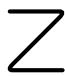
\includegraphics[keepaspectratio]{images/part001_35e3d035.jpg}}

命题 2. 设 \((\mathfrak{g}_i)_{i\in \mathrm{I}}\) 是李代数的一个有限族，且 \(\mathfrak{g} = \prod_{i\in \mathrm{I}}\mathfrak{g}_i\)

\(\mathfrak{g}\) 的嘉当子代数恰是形如 \(\prod_{i\in I}\mathfrak{h}_i\) 的子代数，其中 \(\mathfrak{h}_i\) 是 \(\mathfrak{g}_i\) 的嘉当子代数。

若 \(h_{i}\) 是 \(g_{i}\) 的一个以 \(n_{i}\) 为正规化子的子代数，则 \(\prod h_{i}\) 是 g 的一个以 \(\prod n_{i}\) 为正规化子的子代数；若诸 \(h_{i}\) 幂零，则 \(\prod h_{i}\) 幂零；于是，若对所有 i，\(h_{i}\) 都是 \(g_{i}\) 的嘉当子代数，则 \(\prod h_{i}\) 是 g 的嘉当子代数。反之，设 h 是 g 的一个嘉当子代数；投影 \(h_{i}\) （h 到 \(g_{i}\) 上的）是 \(g_{i}\) 的幂零子代数，且 \(\prod h_{i}\) 是 g 的包含 h 的幂零子代数；故 \(h = \prod h_{i}\) （命题 1）；于是对所有 i，\(h_{i}\) 是它在 \(g_{i}\) 中的自身的正规化子，从而是 \(g_{i}\) 的嘉当子代数。

例 4. 若 k 的特征为 0，则 \(\mathfrak{gl}(n,k)\) 是理想 \(\mathfrak{sl}(n,k)\) 与 k.1 的乘积。由例 2 与命题 2 可知，\(\mathfrak{sl}(n,k)\) 中迹为 0 的对角矩阵所成的集合是 \(\mathfrak{sl}(n,k)\) 的一个嘉当子代数。

命题 3. 设 g 是一个李代数，h 是 g 的一个子代数，\(k'\) 是 k 的一个扩张。那么 h 是 g 的嘉当子代数当且仅当 \(h \otimes_{k} k'\) 是 \(g \otimes_{k} k'\) 的嘉当子代数。

事实上，\(\mathfrak{h}\) 幂零当且仅当 \(\mathfrak{h} \otimes_k k'\) 幂零（第一章，§4，第 5 节）。另一方面，若 \(\mathfrak{n}\) 是 \(\mathfrak{h}\) 在 \(\mathfrak{g}\) 中的正规化子，则 \(\mathfrak{h} \otimes_k k'\) 在 \(\mathfrak{g} \otimes_k k'\) 中的正规化子是 \(\mathfrak{n} \otimes_k k'\) （第一章，§3，第 8 节）。

命题 4. 设 \(\mathfrak{g}\) 是一个李代数，\(\mathfrak{h}\) 是 \(\mathfrak{g}\) 的一个幂零子代数。那么 \(\mathfrak{h}\) 是 \(\mathfrak{g}\) 的嘉当子代数当且仅当 \(\mathfrak{g}^0 (\mathfrak{h}) = \mathfrak{h}\) 。

若 \(\mathfrak{g}^0 (\mathfrak{h}) = \mathfrak{h}\) ，则 \(\mathfrak{h}\) 是它自身的正规化子（§1，命题 10 (i)），故 \(\mathfrak{h}\) 是 \(\mathfrak{g}\) 的嘉当子代数。假定 \(\mathfrak{g}^0 (\mathfrak{h})\neq \mathfrak{h}\) 。考虑由伴随表示转到商而得到的 \(\mathfrak{h}\) 在 \(\mathfrak{g}^0 (\mathfrak{h}) / \mathfrak{h}\) 上的表示。应用 Engel 定理（第一章，§4，第 2 节，定理 1），可见存在 \(x\in \mathfrak{g}^0 (\mathfrak{h})\) 使得 \(x\notin \mathfrak{h}\) 且 \([\mathfrak{h},x]\subset \mathfrak{h}\) ；于是 \(x\) 属于 \(\mathfrak{h}\) 在 \(\mathfrak{g}\) 中的正规化子，故 \(\mathfrak{h}\) 不是 \(\mathfrak{g}\) 的嘉当子代数。

推论 1. 设 \(\mathfrak{g}\) 是一个李代数，\(\mathfrak{h}\) 是 \(\mathfrak{g}\) 的一个嘉当子代数。若 \(k\) 是无限的，则存在 \(x \in \mathfrak{h}\) 使 \(\mathfrak{h} = \mathfrak{g}^0(x)\) 。

事实上，\(\mathfrak{h} = \mathfrak{g}^0 (\mathfrak{h})\) ，故可应用 §1 的命题 9 (ii)。

推论 2. 设 \(f: \mathfrak{g} \to \mathfrak{g}'\) 是李代数的满射同态。若 \(\mathfrak{h}\) 是 \(\mathfrak{g}\) 的嘉当子代数，则 \(f(\mathfrak{h})\) 是 \(\mathfrak{g}'\) 的嘉当子代数。

事实上，\(f(\mathfrak{h})\) 是 \(\mathfrak{g}'\) 的幂零子代数。另一方面，考虑表示 \(x \mapsto \operatorname{ad} f(x)\) ，即 \(\mathfrak{h}\) 在 \(\mathfrak{g}'\) 上的表示。由 §1 第 3 节的命题 9 (iv)，\(f(\mathfrak{g}^0(\mathfrak{h})) = \mathfrak{g}'^0(\mathfrak{h})\) 。而 \(\mathfrak{g}^0(\mathfrak{h}) = \mathfrak{h}\) ，另一方面显然有 \(\mathfrak{g}'^0(\mathfrak{h}) = \mathfrak{g}'^0(f(\mathfrak{h}))\) 。于是 \(f(\mathfrak{h}) = \mathfrak{g}'^0(f(\mathfrak{h}))\) ，只需应用命题 4。

推论 3. 设 \(\mathfrak{h}\) 是李代数 \(\mathfrak{g}\) 的一个嘉当子代数，并设 \(\mathcal{C}^n\mathfrak{g}\) （ \(n \geq 1\) ）是 \(\mathfrak{g}\) 的下降中心列的一项（第一章，§1，第 5 节）。那么 \(\mathfrak{g} = \mathfrak{h} + \mathcal{C}^n\mathfrak{g}\) 。

事实上，推论 2 表明 \(\mathfrak{h}\) 在 \(\mathfrak{g} / \mathcal{C}^n\mathfrak{g}\) 中的像是 \(\mathfrak{g} / \mathcal{C}^n\mathfrak{g}\) 的嘉当子代数，由于 \(\mathfrak{g} / \mathcal{C}^n\mathfrak{g}\) 幂零（例 1），故它等于 \(\mathfrak{g} / \mathcal{C}^n\mathfrak{g}\) 。

推论 4. 设 \(\mathfrak{g}\) 是一个李代数，\(\mathfrak{h}\) 是 \(\mathfrak{g}\) 的一个嘉当子代数，\(\mathfrak{a}\) 是 \(\mathfrak{g}\) 的一个包含 \(\mathfrak{h}\) 的子代数。

\begin{enumerate}
\def\labelenumi{(\roman{enumi})}
\item
  \(\mathfrak{a}\) 等于它在 \(\mathfrak{g}\) 中的自身的正规化子。
\item
  假定 \(k = \mathbf{R}\) 或 \(\mathbf{C}\) ；设 \(G\) 是以 \(\mathfrak{g}\) 为李代数的一个李群，A 是 \(G\) 的以 \(\mathfrak{a}\) 为李代数的积分子群。那么 \(A\) 是 \(G\) 的一个李子群，且它是 \(A\) 在 \(G\) 中的正规化子的单位元连通分支。
\end{enumerate}

设 n 是 a 在 g 中的正规化子。由于 h 是 n 的嘉当子代数（例 3），\(\{0\}\) 是 n/a 的嘉当子代数（推论 2），故等于它在 n/a 中的正规化子；换言之，n = a。断言 (ii) 由 (i) 及第三章，§9，第 4 节，命题 11 的推论得出。

推论 5. 设 g 是一个李代数，E 是 g 的一个子集。让 E 通过伴随表示作用在 g 上。那么 E 是 g 的嘉当子代数当且仅当 \(E = \mathfrak{g}^{0}(E)\) 。

该条件是必要的（命题 4）。现在假定 \(\mathrm{E} = \mathfrak{g}^0 (\mathrm{E})\) 。由 §1 第 1 节的命题 2 (ii)，E 这时是 \(\mathfrak{g}\) 的一个子代数。若 \(x\in \mathrm{E}\) ，则 \(\mathrm{ad}_{\mathrm{E}}x\) 幂零，由于 \(\mathrm{E}\subset \mathfrak{g}^0 (\mathrm{E})\) ；故代数 E 幂零。于是由命题 4，E 是嘉当子代数。

推论 6. 设 g 是一个李代数，\(k_{0}\) 是 k 的一个使 \([k:k_{0}]<+\infty\) 的子域，\(g_{0}\) 是由 g 把纯量域限制到 \(k_{0}\) 而得到的李代数。设 h 是 g 的一个子集。那么 h 是 g 的嘉当子代数当且仅当 h 是 \(g_{0}\) 的嘉当子代数。

这由推论 5 得出，因为条件 \(\mathfrak{h} = \mathfrak{g}^0 (\mathfrak{h})\) 与基域无关。

命题 5. 设 g 是一个李代数，c 是它的中心，h 是 g 的一个向量子空间。那么 h 是 g 的嘉当子代数当且仅当 h 包含 c 且 h/c 是 g/c 的嘉当子代数。

假定 \(\mathfrak{h}\) 是 \(\mathfrak{g}\) 的嘉当子代数。由于 \([\mathfrak{c},\mathfrak{g}]\subset \mathfrak{h}\) ，有 \(\mathfrak{c}\subset \mathfrak{h}\) 。另一方面，由命题 4 的推论 2，\(\mathfrak{h} / \mathfrak{c}\) 是 \(\mathfrak{g} / \mathfrak{c}\) 的嘉当子代数。

假定 \(\mathfrak{h} \supset \mathfrak{c}\) 且 \(\mathfrak{h} / \mathfrak{c}\) 是 \(\mathfrak{g} / \mathfrak{c}\) 的嘉当子代数。设 \(f\) 是从 \(\mathfrak{g}\) 到 \(\mathfrak{g} / \mathfrak{c}\) 的典则态射。代数 \(\mathfrak{h}\) 是 \(\mathfrak{h} / \mathfrak{c}\) 的一个中心扩张，故幂零。设 \(\mathfrak{n}\) 是 \(\mathfrak{h}\) 在 \(\mathfrak{g}\) 中的正规化子。若 \(x \in \mathfrak{n}\) ，则 \([f(x), \mathfrak{h} / \mathfrak{c}] \subset \mathfrak{h} / \mathfrak{c}\) ，故 \(f(x) \in \mathfrak{h} / \mathfrak{c}\) ，从而 \(x \in \mathfrak{h}\) 。这证明 \(\mathfrak{h}\) 是 \(\mathfrak{g}\) 的嘉当子代数。

推论. 设 \(\mathcal{C}_{\infty}\mathfrak{g}\) 是李代数 \(\mathfrak{g}\) 的上升中心列的并（第一章，§1，第 6 节）。\(\mathfrak{g}\) 的嘉当子代数恰是 \(\mathfrak{g}/\mathcal{C}_{\infty}\mathfrak{g}\) 的嘉当子代数的逆像。

事实上，\(\mathfrak{g} / \mathcal{C}_i\mathfrak{g}\) 的中心是 \(\mathcal{C}_{i + 1}\mathfrak{g} / \mathcal{C}_i\mathfrak{g}\) ，用归纳法由命题 5 立即得出该推论。

注. \(C_{\infty}g\) 是使 g/n 的中心为零的最小理想 n；它是 g 的一个特征幂零理想。

\subsection{李代数的正则元}

{[}回忆一下，从现在起假定 \(k\) 是无限的。{]}

设 g 是一个维数为 n 的李代数。~若 \(x \in g\) ，把 ad x 的特征多项式写成如下形式

\[
\det (\mathrm{T} - \operatorname{ad} x) = \sum_ {i = 0} ^ {n} a _ {i} (x) \mathrm{T} ^ {i}, \quad \text { with } a _ {i} (x) \in k.
\]

我们有 \(a_i(x) = (-1)^{n - i}\mathrm{Tr}\left(\bigwedge^{n - i}\operatorname {ad}x\right)\) ，参看~《代数》，第三章，§8，第 11 节。这表明 \(x\mapsto a_i(x)\) 是一个 \(n - i\) 次齐次多项式映射，从 \(\mathfrak{g}\) 到 \(k\) （《代数》，第四章，§5，第 9 节）。

注. 1) 若 \(\mathfrak{g} \neq \{0\}\) ，则 \(a_0 = 0\) ，由于 (ad \(x(x) = 0\) 对所有 \(x \in \mathfrak{g}\) 成立。

\begin{enumerate}
\def\labelenumi{\arabic{enumi})}
\setcounter{enumi}{1}
\tightlist
\item
  设 \(k'\) 是 \(k\) 的一个扩张。写 \(\det(\mathrm{T} - \operatorname{ad} x') = \sum_{i=0}^{n} a_i'(x') \mathrm{T}^i\) ，对 \(x' \in \mathfrak{g} \otimes_k k'\) 。那么 \(a_i'| \mathfrak{g} = a_i\) 对所有 \(i\) 成立。
\end{enumerate}

定义 2. g 的秩，记作 rk(g)，是使 \(a_{l} \neq 0\) 的最小整数 l。g 的元素 x 称为正则元，如果 \(a_{l}(x) \neq 0\) 。

对所有 \(x \in \mathfrak{g}\) 有 \(\operatorname{rk}(\mathfrak{g}) \leq \dim \mathfrak{g}^0(x)\) ，且等式成立当且仅当 \(x\) 正则。

正则元之集在 \(\mathfrak{g}\) 中按 Zariski 拓扑是稠密且开的（附录 I）。

例. 1) 若 g 幂零，则 rk(g) = dim g，且 g 的所有元素都正则。

\begin{enumerate}
\def\labelenumi{\arabic{enumi})}
\setcounter{enumi}{1}
\tightlist
\item
  设 \(\mathfrak{g} = \mathfrak{sl}(2,k)\) 。若 \(x = \begin{pmatrix} \gamma & \alpha \\ \beta & -\gamma \end{pmatrix} \in \mathfrak{g}\) ，简单计算给出
\end{enumerate}

\[
\det (\mathrm{T} - \operatorname{ad} x) = \mathrm{T} ^ {3} - 4 (\alpha \beta + \gamma^ {2}) \mathrm{T}.
\]

若 \(k\) 的特征数 \(\neq 2\) ，则 \(\mathrm{rk}(\mathfrak{g}) = 1\) ，且正则元是那些 \(x\) ，使 \(\alpha \beta + \gamma^2 \neq 0\) 。

\begin{enumerate}
\def\labelenumi{\arabic{enumi})}
\setcounter{enumi}{2}
\tightlist
\item
  设 V 是一个有限维为 n 的向量空间，\(\mathfrak{g} = \mathfrak{gl}(V)\) 。设 \(\overline{k}\) 是 k 的一个代数闭包。设 \(x \in g\) ，并设 \(\lambda_{1}, \ldots, \lambda_{n}\) 是 x 的特征多项式在 \(\overline{k}\) 中的根（每个根写出的次数等于其重数）。从 \(V^{*} \otimes V\) 到 g 的典则同构与这两个空间的 g-模结构相容，换言之，它把 \(1 \otimes x - {}^{t}x \otimes 1\) 映到 ad x（第一章，§3，第 3 节，命题 4）。注意到 §1 命题 4 (i)，由此推出 ad x 的特征多项式的根是 \(\lambda_{i} - \lambda_{j}\) ，其中 \(1 \leq i \leq n, 1 \leq j \leq n\) （每个根写出的次数等于其重数）。于是，g 的秩是 n，且 x 正则当且仅当每个 \(\lambda_{i}\) 是 x 的特征多项式的单根。
\end{enumerate}

命题 6. 设 \(\mathfrak{g}\) 是一个李代数，\(k'\) 是 \(k\) 的一个扩张，\(\mathfrak{g}' = \mathfrak{g} \otimes_k k'\) 。

\begin{enumerate}
\def\labelenumi{(\roman{enumi})}
\tightlist
\item
  一个元素 \(x\) （属于 \(\mathfrak{g}\) ）在 \(\mathfrak{g}\) 中正则当且仅当 \(x \otimes 1\) 在 \(\mathfrak{g}'\) 中正则。\\
\item
  \(\operatorname{rk}(\mathfrak{g}) = \operatorname{rk}(\mathfrak{g}')\) 。
\end{enumerate}

这由注 2 得出。

命题 7. 设 \((\mathfrak{g}_i)_{i\in \mathrm{I}}\) 是一个有限的李代数族，\(\mathfrak{g} = \prod_{i\in \mathrm{I}}\mathfrak{g}_i\) 。

\begin{enumerate}
\def\labelenumi{(\roman{enumi})}
\tightlist
\item
  一个元素 \((x_{i})_{i\in \mathrm{I}}\) （属于 \(\mathfrak{g}\) ）在 \(\mathfrak{g}\) 中正则当且仅当对所有 \(i\in \mathrm{I}\) ，\(x_{i}\) 在 \(\mathfrak{g}_i\) 中正则。
\end{enumerate}

\[
\text {(ii)} \operatorname{rk} (\mathfrak {g}) = \sum_ {i \in I} \operatorname{rk} (\mathfrak {g} _ {i}).
\]

事实上，对任意 \(x = (x_{i})_{i \in \mathrm{I}} \in \mathfrak{g}\) ，\(ad_{g}x\) 的特征多项式是诸 \(ad_{g_{i}}x_{i}\) 的特征多项式的乘积。

命题 8. 设 \(f: \mathfrak{g} \to \mathfrak{g}'\) 是李代数的一个满射同态。

\begin{enumerate}
\def\labelenumi{(\roman{enumi})}
\item
  若 \(x\) 是 \(\mathfrak{g}\) 的正则元，则 \(f(x)\) 在 \(\mathfrak{g}'\) 中正则。若 \(\operatorname{Ker} f\) 包含在 \(\mathfrak{g}\) 的中心中，则逆命题成立。
\item
  \(\operatorname{rk}(\mathfrak{g}) \geq \operatorname{rk}(\mathfrak{g}')\) 。
\end{enumerate}

设 \(\mathrm{rk}(\mathfrak{g}) = r, \mathrm{rk}(\mathfrak{g}') = r'\) 。设 \(x \in \mathfrak{g}\) 。\(\operatorname{ad} x\) 、\(\operatorname{ad} f(x)\) 和 \(\operatorname{ad} x|\operatorname{Ker} f\) 的特征多项式形如

\[
\mathrm{P} (\mathrm{T}) = \mathrm{T} ^ {n} + a _ {n - 1} (x) \mathrm{T} ^ {n - 1} + \dots + a _ {r} (x) \mathrm{T} ^ {r},
\]

\[
\mathrm{Q} (\mathrm{T}) = \mathrm{T} ^ {n ^ {\prime}} + b _ {n ^ {\prime} - 1} (x) \mathrm{T} ^ {n ^ {\prime} - 1} + \dots + b _ {r ^ {\prime}} (x) \mathrm{T} ^ {r ^ {\prime}},
\]

\[
\mathrm{R} (\mathrm{T}) = \mathrm{T} ^ {n ^ {\prime \prime}} + c _ {n ^ {\prime \prime} - 1} (x) \mathrm{T} ^ {n ^ {\prime \prime} - 1} + \dots + c _ {r ^ {\prime \prime}} (x) \mathrm{T} ^ {r ^ {\prime \prime}},
\]

其中 \(a_i, b_i, c_i\) 是 \(\mathfrak{g}\) 上的多项式函数，且 \(a_r \neq 0\) ，\(b_{r'} \neq 0\) ，\(c_{r''} \neq 0\) 。我们有 \(\mathrm{P} = \mathrm{QR}\) ，故 \(r = r' + r''\) 且 \(a_r(x) = b_{r'}(x)c_{r''}(x)\) ，这就证明了 (ii) 以及 (i) 的第一个断言。若 \(\operatorname{Ker} f\) 包含在 \(\mathfrak{g}\) 的中心中，则 \(\mathrm{R(T)} = \mathrm{T}^{n''}\) ，从而 \(a_r(x) = b_{r'}(x)\) ，于是得到 (i) 的第二个断言。

推论. 设 \(\mathcal{C}_n\mathfrak{g}\) ( \(n \geq 0\) ) 是 \(\mathfrak{g}\) 的上升中心列的一项（第一章，§1，第 6 节）。\(\mathfrak{g}\) 的正则元是那些在 \(\mathfrak{g}/\mathcal{C}_n\mathfrak{g}\) 中的像正则的元素。

命题 9. 设 \(\mathfrak{g}\) 是一个李代数，\(\mathfrak{g}'\) 是 \(\mathfrak{g}\) 的一个子代数。\(\mathfrak{g}'\) 的每个在 \(\mathfrak{g}\) 中正则的元素在 \(\mathfrak{g}'\) 中正则。

对 \(x \in g'\) ，\(ad_{g}x\) 在 \(g'\) 上的限制是 \(ad_{g'}x\) ，从而通过转到商定义自同态 \(u(x)\) 于向量空间 \(g/g'\) 上。设 \(d_{0}(x)\) （相应地 \(d_{1}(x)\) ）是 \(ad_{g'}(x)\) （相应地 \(u(x)\) ）的幂零空间的维数，并设 \(c_{0}\) （相应地 \(c_{1}\) ）是 \(d_{0}(x)\) （相应地 \(d_{1}(x)\) ）当 x 属于 \(g'\) 时的最小值。存在非零多项式映射 \(p_{0}, p_{1}\) ，从 \(g'\) 到 k，使得

\[
d _ {0} (x) = c _ {0} \Longleftrightarrow p _ {0} (x) \neq 0, \quad d _ {1} (x) = c _ {1} \Longleftrightarrow p _ {1} (x) \neq 0.
\]

由于 k 无限，\(x \in g'\) 中使 \(d_{0}(x) = c_{0}\) 且 \(d_{1}(x) = c_{1}\) 的元素所成的集 S 非空。S 的每个元素在 \(g'\) 中正则。另一方面，S 是 \(g'\) 中使 \(ad_{g}x\) 的幂零空间有最小维数的元素之集，因而包含 \(g'\) 的每个在 g 中正则的元素。

注. 3) \(\mathfrak{g}'\) 的在 \(\mathfrak{g}\) 中正则的元素不一定存在。若至少存在一个，则这些元素之集正是上面证明中记作 S 的集合。

\subsection{嘉当子代数与正则元}

定理 1. 设 \(\mathfrak{g}\) 是一个李代数。

\begin{enumerate}
\def\labelenumi{(\roman{enumi})}
\item
  若 \(x\) 是 \(\mathfrak{g}\) 的正则元，则 \(\mathfrak{g}^0(x)\) 是 \(\mathfrak{g}\) 的嘉当子代数。
\item
  若 \(\mathfrak{h}\) 是 \(\mathfrak{g}\) 的一个极大幂零子代数，且 \(x \in \mathfrak{h}\) 在 \(\mathfrak{g}\) 中正则，则 \(\mathfrak{h} = \mathfrak{g}^0(x)\) 。
\item
  若 \(\mathfrak{h}\) 是 \(\mathfrak{g}\) 的嘉当子代数，则 \(\dim (\mathfrak{h})\geq \mathrm{rk}(\mathfrak{g})\)
\item
  \(\mathfrak{g}\) 的维数为 \(\mathrm{rk}(\mathfrak{g})\) 的嘉当子代数恰是诸 \(\mathfrak{g}^0 (x)\) ，其中 \(x\) 是正则元。
\end{enumerate}

设 \(x\) 是 \(\mathfrak{g}\) 的正则元，并设 \(\mathfrak{h} = \mathfrak{g}^0(x)\) 。显然 \(\mathfrak{h}^0(x) = \mathfrak{h}\) 。由于 \(x\) 在 \(\mathfrak{h}\) 中正则（命题 9），\(\operatorname{rk}(\mathfrak{h}) = \dim(\mathfrak{h})\) ，故 \(\mathfrak{h}\) 幂零。另一方面，\(\mathfrak{h} = \mathfrak{g}^0(x) \supset \mathfrak{g}^0(\mathfrak{h}) \supset \mathfrak{h}\) ，故 \(\mathfrak{h} = \mathfrak{g}^0(\mathfrak{h})\) 是 \(\mathfrak{g}\) 的嘉当子代数（命题 4）。这就证明了 (i)。

若 \(\mathfrak{h}\) 是 \(\mathfrak{g}\) 的一个极大幂零子代数，且 \(x\in \mathfrak{h}\) 在 \(\mathfrak{g}\) 中正则，则 \(\mathfrak{h}\subset \mathfrak{g}^0 (x)\) ，且由 (i) \(\mathfrak{g}^0 (x)\) 幂零，故 \(\mathfrak{h} = \mathfrak{g}^0 (x)\) ，这就证明了 (ii)。

若 \(\mathfrak{h}\) 是 \(\mathfrak{g}\) 的嘉当子代数，则存在 \(x \in \mathfrak{h}\) 使 \(\mathfrak{h} = \mathfrak{g}^0(x)\) （命题 4 的推论 1），故 \(\dim(\mathfrak{h}) \geq \operatorname{rk}(\mathfrak{g})\) ，这就证明了 (iii)。若此外 \(\dim(\mathfrak{h}) = \operatorname{rk}(\mathfrak{g})\) ，则 \(x\) 正则。最后，若 \(x'\) 在 \(\mathfrak{g}\) 中正则，则由 (i) \(\mathfrak{g}^0(x')\) 是嘉当子代数，且显然维数为 \(\operatorname{rk}(\mathfrak{g})\) 。这就证明了 (iv)。

我们将在 §3 定理 2 中看到，当 \(k\) 的特征数为零时，\(\mathfrak{g}\) 的所有嘉当子代数都有维数 \(\mathrm{rk}(\mathfrak{g})\) 。

推论 1. 每个李代数 g 都有嘉当子代数，且 g 的秩是嘉当子代数的最小维数。

推论 2. 设 \(f: \mathfrak{g} \to \mathfrak{g}'\) 是李代数的一个满射同态。若 \(\mathfrak{h}'\) 是 \(\mathfrak{g}'\) 的嘉当子代数，则存在一个嘉当子代数 \(\mathfrak{h}\) （在 \(\mathfrak{g}\) 中）使 \(\mathfrak{h}' = f(\mathfrak{h})\) 。

设 \(\mathfrak{a} = f^{-1}(\mathfrak{h}')\) 。由推论 1，\(\mathfrak{a}\) 有一个嘉当子代数 \(\mathfrak{h}\) 。由命题 4 的推论 2，\(f(\mathfrak{h}) = \mathfrak{h}'\) 。我们证明 \(\mathfrak{h}\) 是 \(\mathfrak{g}\) 的嘉当子代数。设 \(\mathfrak{n}\) 是 \(\mathfrak{h}\) 在 \(\mathfrak{g}\) 中的正规化子。只需证明 \(\mathfrak{h} = \mathfrak{n}\) 。若 \(x \in \mathfrak{n}\) ，则 \(f(x)\) 属于 \(\mathfrak{h}'\) 在 \(\mathfrak{g}'\) 中的正规化子，故 \(f(x) \in \mathfrak{h}'\) 且 \(x \in \mathfrak{a}\) ；但 \(\mathfrak{h}\) 在 \(\mathfrak{a}\) 中是自身的正规化子，故 \(x \in \mathfrak{h}\) 。

推论 3. 每个李代数 \(\mathfrak{g}\) 都是它的嘉当子代数之和。

g 的诸嘉当子代数之和 s 包含 g 的正则元之集（定理 1 (i)）。由于该集在 g 中按 Zariski 拓扑稠密，故 s = g。

命题 10. 设 g 是一个李代数，a 是 g 的一个交换子代数，c 是 a 在 g 中的交换子。假定 \(ad_{g}x\) 对所有 \(x \in a\) 半单。那么 c 的嘉当子代数恰是 g 的包含 a 的嘉当子代数。

设 \(\mathfrak{h}\) 是 \(\mathfrak{c}\) 的嘉当子代数。由于 \(\mathfrak{a}\) 包含在中心 \(\mathfrak{z}\) 中，即有 \(\mathfrak{c}, \mathfrak{a} \subset \mathfrak{z} \subset \mathfrak{h}\) （命题 5）。设 \(\mathfrak{n}\) 是 \(\mathfrak{h}\) 在 \(\mathfrak{g}\) 中的正规化子。那么

\[
[ \mathfrak {a}, \mathfrak {n} ] \subset [ \mathfrak {h}, \mathfrak {n} ] \subset \mathfrak {h}.
\]

由于诸 \(ad_{g}x\) （\(x \in a\) ）半单且两两交换，由《代数》第八章 §5 第 1 节可知，存在 n 的一个在 \(ad_{g}a\) 下稳定的向量子空间 d 使得 \(n = h \oplus d\) 。于是 \([a, d] \subset h \cap d = 0\) ，故 \(d \subset c\) 。从而 n 是 h 在 c 中的正规化子，因此 \(n = h\) ，故 h 是 g 的包含 a 的嘉当子代数。

反过来，设 \(\mathfrak{h}\) 是 \(\mathfrak{g}\) 的包含 \(\mathfrak{a}\) 的嘉当子代数。那么 \(\mathfrak{h} = \mathfrak{g}^0 (\mathfrak{h})\subset \mathfrak{g}^0 (\mathfrak{a})\) ，且由假定 \(\mathfrak{g}_0(\mathfrak{a}) = \mathfrak{g}^0 (\mathfrak{a}) = \mathfrak{c}\) 。因此 \(\mathfrak{a}\subset \mathfrak{h}\subset \mathfrak{c}\) ，且 \(\mathfrak{h}\) 是 \(\mathfrak{c}\) 的嘉当子代数（因为它在 \(\mathfrak{g}\) 中等于自身的正规化子，故在 \(\mathfrak{c}\) 中更其如此）。

命题 11. 设 \(\mathfrak{n}\) 是李代数 \(\mathfrak{g}\) 的一个幂零子代数。存在 \(\mathfrak{g}\) 的一个包含于 \(\mathfrak{g}^0 (\mathfrak{n})\) 的嘉当子代数。

设 \(\mathfrak{a} = \mathfrak{g}^0 (\mathfrak{n})\) 。于是 \(\mathfrak{n}\subset \mathfrak{a}\) ，由于 \(\mathfrak{n}\) 幂零。若 \(x\in \mathfrak{a}\) ，设 \(\mathrm{P}(x)\) 是 \(\mathfrak{g} / \mathfrak{a}\) 的自同态（由 ad \(x\) 定义）的行列式。用 \(\mathfrak{a}'\) 记 \(x\in \mathfrak{a}\) 中使 \(\mathrm{P}(x)\neq 0\) 者所成之集，它是 \(\mathfrak{a}\) 中按 Zariski 拓扑的一个开子集；关系 \(x\in \mathfrak{a}'\) 与 \(\mathfrak{g}^0 (x)\subset \mathfrak{a}\) 等价。由 §1 第 2 节的命题 7 (ii)，存在 \(y\in \mathfrak{n}\) 使 \(\mathfrak{g}^0 (y) = \mathfrak{a}\) ，且 \(y\in \mathfrak{a}'\) ，故 \(\mathfrak{a}'\) 非空。由于 \(\mathfrak{a}'\) 开，它与 \(\mathfrak{a}\) 的正则元之集的交非空。设 \(x\) 是该交中的一个元素。那么 \(\mathfrak{g}^0 (x)\subset \mathfrak{a}\) ，且 \(\mathfrak{g}^0 (x)\) 是 \(\mathfrak{a}\) 的嘉当子代数，故幂零。另一方面，§1 第 3 节的命题 10 (i) 表明 \(\mathfrak{g}^0 (x)\) 在 \(\mathfrak{g}\) 中是自身的正规化子；因此它是 \(\mathfrak{g}\) 的嘉当子代数，证毕。

\subsection{半单李代数的嘉当子代数}

定理 2. 假定 k 的特征数为 0。设 g 是一个半单李代数，h 是 g 的嘉当子代数。那么 h 交换，且它的所有元素在 g 中半单（第一章，§6，第 3 节，定义 3）。

由于 \(\mathfrak{h} = \mathfrak{g}^0 (\mathfrak{h})\) ，\(\mathfrak{h}\) 约化（§1，命题 11），又因它幂零故交换。另一方面，\(\mathfrak{g}\) 的伴随表示在 \(\mathfrak{h}\) 上的限制半单（同处所引），故 \(\mathfrak{h}\) 的元素在 \(\mathfrak{g}\) 中半单（《代数》，第八章，§5，第 1 节）。

推论 1. 若 \(x \in \mathfrak{h}\) 且 \(y \in \mathfrak{g}^{\lambda}(\mathfrak{h})\) ，我们有 \([x, y] = \lambda(x)y\) 。

事实上，\(\mathfrak{g}^{\lambda (x)}(x) = \mathfrak{g}_{\lambda (x)}(x)\) ，由于 ad \(x\) 半单。

推论 2. g 的每个正则元半单。

事实上，这样的元素属于某个嘉当子代数（第 3 节，定理 1 (i)）。

推论 3. 设 \(\mathfrak{h}\) 是约化李代数 \(\mathfrak{g}\) 的嘉当子代数。a) \(\mathfrak{h}\) 交换。

\begin{enumerate}
\def\labelenumi{\alph{enumi})}
\setcounter{enumi}{1}
\tightlist
\item
  若 \(\rho\) 是 \(\mathfrak{g}\) 的一个有限维半单表示，则 \(\rho(\mathfrak{h})\) 的元素半单。
\end{enumerate}

设 \(\mathfrak{c}\) 是 \(\mathfrak{g}\) 的中心，\(\mathfrak{s}\) 是它的导代数。那么 \(\mathfrak{g} = \mathfrak{c} \times \mathfrak{s}\) ，故 \(\mathfrak{h} = \mathfrak{c} \times \mathfrak{h}'\) ，其中 \(\mathfrak{h}'\) 是 \(\mathfrak{s}\) 的嘉当子代数（命题 2）。注意到定理 2，\(\mathfrak{h}'\) 交换，故 \(\mathfrak{h}\) 亦然。此外，\(\rho(\mathfrak{h}')\) 由半单元素组成，\(\rho(\mathfrak{c})\) 亦然（第一章，§6，第 5 节，定理 4）；由此得到断言 \(b\) )。

\section{共轭定理}

在本段中，基域 \(k\) 的特征数为 0。

\subsection{初等自同构}

设 \(\mathfrak{g}\) 是一个李代数。用 \(\operatorname{Aut}(\mathfrak{g})\) 记它的自同构群。若 \(x \in \mathfrak{g}\) 且 \(\operatorname{ad} x\) 幂零，则 \(e^{\operatorname{ad} x} \in \operatorname{Aut}(\mathfrak{g})\) （第一章，§6，第 8 节）。

定义 1. g 的形如 \(e^{ad x}\) （其中 ad x 幂零）的自同构的有限积称为 g 的初等自同构。g 的初等自同构群记作 \(\operatorname{Aut}_{e}(\mathfrak{g})\) 。

若 \(u \in \operatorname{Aut}(\mathfrak{g})\) ，则 \(ue^{\operatorname{ad}x}u^{-1} = e^{\operatorname{ad}u(x)}\) 。由此推出 \(\operatorname{Aut}_{e}(\mathfrak{g})\) 是 \(\operatorname{Aut}(\mathfrak{g})\) 的一个正规子群。若 k = R 或 C，则 \(\operatorname{Aut}_{e}(\mathfrak{g})\) 包含在 g 的内自同构群 \(\operatorname{Int}(\mathfrak{g})\) 中（第三章，§6，第 2 节，定义 2）。

* 在一般情形，\(\mathrm{Aut}_e(\mathfrak{g})\) 包含在代数群 \(\mathrm{Aut}(\mathfrak{g})\) 的单位元连通分支中。*

引理 1. 设 \(\mathrm{V}\) 是一个有限维向量空间，\(\mathfrak{n}\) 是 \(\mathfrak{a} = \mathfrak{gl}(\mathrm{V})\) 的一个由幂零元素组成的李子代数。

\begin{enumerate}
\def\labelenumi{(\roman{enumi})}
\item
  映射 \(x \mapsto \exp x\) 是从 \(\mathfrak{n}\) 到子群 \(N\) （\(\mathbf{GL}(V)\) 的，由幺幂元素组成）的双射（第二章，§6，第 1 节，注 4）。我们有 \(\mathfrak{n} = \log(\exp \mathfrak{n})\) 。映射 \(f \mapsto f \circ \log\) 是从 \(\mathfrak{n}\) 上的多项式函数代数到 \(\mathbf{N}\) 上的限制所成的代数（\(\operatorname{End}(\mathbf{V})\) 上的多项式函数的限制）的同构。
\item
  若 \(x \in \mathfrak{n}\) 且 \(a \in \mathfrak{a}\) ，则
\end{enumerate}

\[
(\exp \operatorname{ad} _ {\mathfrak {a}} x). a = (\exp x) a (\exp (- x)).
\]

\begin{enumerate}
\def\labelenumi{(\roman{enumi})}
\setcounter{enumi}{2}
\tightlist
\item
  设 \(V'\) 是一个有限维向量空间，\(n'\) 是 \(\mathfrak{gl}(V')\) 的一个由幂零元素组成的李子代数，\(\rho\) 是从 n 到 \(n'\) 的一个同态。设 \(\pi\) 是映射 \(\exp x \mapsto \exp \rho(x)\) （从 \(\exp n\) 到 \(\exp n'\) ）。那么 \(\pi\) 是一个群同态。
\end{enumerate}

由 Engel 定理，可以把 V 与 \(k^n\) 等同起来，使 \(\mathfrak{n}\) 是 \(\mathfrak{n}(n,k)\) （由对角线上为零的下三角矩阵组成的 \(\mathbf{M}_n(k)\) 的李子代数）的一个子代数。对 \(s \geq 0\) ，设 \(\mathfrak{n}_s(n,k)\) 是 \((x_{ij})_{1 \leq i,j \leq n} \in \mathbf{M}_n(k)\) 中使 \(x_{ij} = 0\) （对 \(i - j < s\) ）者所成之集。那么

\[
[ \mathfrak {n} _ {s} (n, k), \mathfrak {n} _ {s ^ {\prime}} (n, k) ] \subset \mathfrak {n} _ {s + s ^ {\prime}} (n, k)
\]

（第二章，§4，第 6 节，注），且 Hausdorff 级数定义了一个多项式映射 \((a,b)\mapsto\mathrm{H}(a,b)\) ，从 \(\mathfrak{n}(n,k)\times\mathfrak{n}(n,k)\) 到 \(\mathfrak{n}(n,k)\) （第二章，§6，第 5 节，注 3）；该映射使 \(\mathfrak{n}(n,k)\) 成为一个群（第二章，§6，第 5 节，命题 4）。由第二章 §6 第 1 节注 4，映射 \(x\mapsto\exp x\) （从 \(\mathfrak{n}(n,k)\) 到 \(1+\mathfrak{n}(n,k)\) ）与映射 \(y\mapsto\log y\) （从 \(1+\mathfrak{n}(n,k)\) 到 \(\mathfrak{n}(n,k)\) ）是互逆的双射且都是多项式的；由第二章 §6 第 5 节命题 3，若给 \(\mathfrak{n}(n,k)\) 赋予群律 \((a,b)\mapsto\mathrm{H}(a,b)\) ，并把 \(1+\mathfrak{n}(n,k)\) 视为 \(\mathbf{GL}_{n}(k)\) 的子群，则这些映射是群同构。于是引理的断言 (i) 和 (iii) 得出。设 \(x\in\mathfrak{n}\) 。用 \(\mathrm{L}_{x},\mathrm{R}_{x}\) 记映射 \(u\mapsto xu,u\mapsto ux\) （从 \(\mathfrak{a}\) 到 \(\mathfrak{a}\) ），它们交换且幂零。我们有 \(\mathrm{ad}_{\mathfrak{a}}x=\mathrm{L}_{x}-\mathrm{R}_{x}\) ，故对所有 \(a\in\mathfrak{a}\) ，

\[
\begin{array}{c} (\exp \operatorname{ad} _ {\mathfrak {a}} x) a = (\exp (\mathrm{L} _ {x} - \mathrm{R} _ {x})) a = (\exp \mathrm{L} _ {x}) (\exp \mathrm{R} _ {- x}) a \\ = \sum_ {i, j \geq 0} \frac {\mathrm{L} _ {x} ^ {i}}{i !} \frac {\mathrm{R} _ {- x} ^ {j}}{j !} a = (\exp x) a (\exp (- x)). \end{array}\tag{1}
\]

用引理 1 中的记号，\(\pi\) 称为 \(\exp \mathfrak{n}\) 的与给定表示 \(\rho\) （\(\mathfrak{n}\) 在 \(V'\) 上的）相容的线性表示。当 \(k\) 是 \(\mathbf{R}\) 、\(\mathbf{C}\) 或一个非离散完备超度量域时，由指数映射的性质有 \(\rho = L(\pi)\) （第三章，§4，第 4 节，命题 8 的推论 2）。

命题 1. 设 \(\mathfrak{g}\) 是一个李代数，\(\mathfrak{n}\) 是 \(\mathfrak{g}\) 的一个使 \(\operatorname{ad}_{\mathfrak{g}}x\) 对所有 \(x\in \mathfrak{n}\) 幂零的子代数。那么 \(e^{\operatorname{ad}_{\mathfrak{g}}\mathfrak{n}}\) 是 \(\operatorname{Aut}_e(\mathfrak{g})\) 的一个子群。

这由引理 1 (i) 立即得出。

特别地，若 \(\mathfrak{n}\) 是 \(\mathfrak{g}\) 的幂零根基，则 \(e^{\mathrm{ad}_{\mathfrak{g}}\mathfrak{n}}\) 是 \(\mathfrak{g}\) 的特殊自同构群（第一章，§6，第 8 节，定义 6）。

注. 1) 设 V 是一个有限维向量空间，g 是 \(\mathfrak{a} = \mathfrak{gl}(V)\) 的一个李子代数，x 是 g 的一个使 \(ad_{g}x\) 幂零的元素。那么存在 a 的一个幂零元素 n 使 \(ad_{a}n\) 延拓 \(ad_{g}x\) 。事实上，设 s, n 是 x 的半单分量与幂零分量；那么 \(ad_{a}s\) 和 \(ad_{a}n\) 是 \(ad_{a}x\) 的半单分量与幂零分量（第一章，§5，第 4 节，引理 2），故 \(ad_{a}s\) 和 \(ad_{a}n\) 保持 g 稳定，且 \(ad_{a}s|g\) 和 \(ad_{a}n|g\) 是 \(ad_{g}x\) 的半单分量与幂零分量；因此 \(ad_{g}x = ad_{a}n|g\) ，这就证明了我们的断言。注意到引理 1 (ii)，g 的每个初等自同构都延拓为 a 的一个形如 \(u \mapsto mum^{-1}\) （其中 \(m \in \mathbf{GL}(V)\) ）的自同构。

\begin{enumerate}
\def\labelenumi{\arabic{enumi})}
\setcounter{enumi}{1}
\tightlist
\item
  设 V 是一个有限维向量空间。对每个 \(g \in \mathbf{SL}(V)\) ，用 \(\varphi(g)\) 记自同构 \(x \mapsto gxg^{-1}\) （\(\mathfrak{gl}(V)\) 的）。那么
\end{enumerate}

\[
\operatorname{Aut} _ {e} (\mathfrak {g l} (V)) = \varphi (\mathbf {S L} (V)).
\]

事实上，由 (1)，\(\operatorname{Aut}_{e}(\mathfrak{gl}(V))\) 包含在 \(\varphi(\mathbf{SL}(V))\) 中，而反向包含由《代数》第三章 §8 第 9 节命题 17 及 (1) 得出。类似的论证表明 \(\operatorname{Aut}_{e}(\mathfrak{sl}(V))\) 是 \(\varphi(\mathbf{SL}(V))\) 的元素在 \(\mathfrak{sl}(V)\) 上的限制所成之集。

\subsection{嘉当子代数的共轭性}

设 g 是一个李代数，h 是 g 的一个幂零子代数，R 是 h 在 g 中的非零权之集，换言之，是 h 上的线性形式 \(\lambda \neq 0\) 中使 \(\mathfrak{g}^{\lambda}(\mathfrak{h}) \neq 0\) 者所成之集，参看~§1 第 3 节命题 9 (iii)。假定

\[
\mathfrak {g} = \mathfrak {g} ^ {0} (\mathfrak {h}) \oplus \sum_ {\lambda \in R} \mathfrak {g} ^ {\lambda} (\mathfrak {h}),
\]

当 \(k\) 代数闭时即为此情形（§1，第 3 节，命题 9 (i)）。对 \(\lambda \in \mathbb{R}\) 和 \(x \in \mathfrak{g}^{\lambda}(\mathfrak{h})\) ，ad \(x\) 幂零（§1，第 3 节，命题 10 (iv)）。用 \(\mathrm{E}(\mathfrak{h})\) 记 \(\mathrm{Aut}_e(\mathfrak{g})\) 的由诸 \(e^{\mathrm{ad}x}\) （其中 \(x\) 形如上面）生成的子群。若 \(u \in \mathrm{Aut}(\mathfrak{g})\) ，立即有 \(u\mathrm{E}(\mathfrak{h})u^{-1} = \mathrm{E}(u(\mathfrak{h}))\) 。

引理 2. (i) 设 \(\mathfrak{h}_r\) 是 \(x\in \mathfrak{h}\) 中使 \(\mathfrak{g}^0 (x) = \mathfrak{g}^0 (\mathfrak{h})\) 者所成之集；这是 \(x\in \mathfrak{h}\) 中使 \(\lambda (x)\neq 0\) 对所有 \(\lambda \in \mathrm{R}\) 成立者所成之集，且 \(\mathfrak{h}_r\) 在 \(\mathfrak{h}\) 中按 Zariski 拓扑既开又稠密。

\begin{enumerate}
\def\labelenumi{(\roman{enumi})}
\setcounter{enumi}{1}
\tightlist
\item
  设 \(R = \{\lambda_{1}, \lambda_{2}, \ldots, \lambda_{p}\}\) ，其中诸 \(\lambda_{i}\) 两两不同。设 F 是从 \(\mathfrak{g}^{0}(\mathfrak{h}) \times \mathfrak{g}^{\lambda_{1}}(\mathfrak{h}) \times \cdots \times \mathfrak{g}^{\lambda_{p}}(\mathfrak{h})\) 到 g 的由公式
\end{enumerate}

\[
\mathrm{F} (h, x _ {1}, \dots , x _ {p}) = e ^ {\operatorname{ad} x _ {1}} \dots e ^ {\operatorname{ad} x _ {p}} h.
\]

定义的映射。那么 \(\mathrm{F}\) 是一个支配多项式映射（附录 I）。

断言 (i) 是明显的。我们证明 (ii)。设 \(n = \dim \mathfrak{g}\) 。若 \(\lambda \in \mathrm{R}\) 且 \(x \in \mathfrak{g}^{\lambda}(\mathfrak{h})\) ，我们有 \((\operatorname{ad} x)^n = 0\) 。由此推出 \((y, x) \mapsto e^{\operatorname{ad} x} y\) 是从 \(\mathfrak{g} \times \mathfrak{g}^{\lambda}(\mathfrak{h})\) 到 \(\mathfrak{g}\) 的多项式映射；用归纳法推出 \(\mathrm{F}\) 是多项式的。设 \(h_0 \in \mathfrak{h}_r\) ，并设 \(\mathrm{DF}\) 是 \(\mathrm{F}\) 在 \((h_0, 0, \ldots, 0)\) 处的切线性映射；我们证明 \(\mathrm{DF}\) 满射。对 \(h \in \mathfrak{g}^{0}(\mathfrak{h})\) ，有 \(F(h_{0} + h, 0, \ldots, 0) = h_{0} + h\) ，故 \(\mathrm{DF}(h, 0, \ldots, 0) = h\) ，从而 \(\mathrm{Im}(\mathrm{DF}) \supset \mathfrak{g}^{0}(\mathfrak{h})\) 。另一方面，对 \(x \in \mathfrak{g}^{\lambda_{1}}(\mathfrak{h})\) ，

\[
\mathrm{F} (h _ {0}, x, 0, \dots , 0) = e ^ {\operatorname{ad} x} h _ {0} = h _ {0} + (\operatorname{ad} x). h _ {0} + \frac {(\operatorname{ad} x) ^ {2}}{2 !} h _ {0} + \dots
\]

故 \(\mathrm{DF}(0,x,0,\ldots ,0) = (\mathrm{ad}x).h_0 = -(\mathrm{ad}h_0)x\) ；由于 \(\mathrm{ad}h_0\) 诱导 \(\mathfrak{g}^{\lambda_1}(\mathfrak{h})\) 的一个自同构，\(\operatorname {Im}(\mathrm{DF})\supset \mathfrak{g}^{\lambda_1}(\mathfrak{h})\) 。类似地，

\[
\operatorname{Im} (\mathrm{DF}) \supset \mathfrak {g} ^ {\lambda_ {i}} (\mathfrak {h})
\]

对所有 \(i\) 成立，故 DF 满射。于是附录 I 的命题 4 表明 F 是支配的。

命题 2. 假定 \(k\) 代数闭。设 \(\mathfrak{g}\) 是一个李代数，\(\mathfrak{h}\) 和 \(\mathfrak{h}'\) 是 \(\mathfrak{g}\) 的嘉当子代数。存在 \(u \in \mathrm{E}(\mathfrak{h})\) 和 \(u' \in \mathrm{E}(\mathfrak{h}')\) 使 \(u(\mathfrak{h}) = u'(\mathfrak{h}')\) 。

我们保留引理 2 的记号。由 \(\mathfrak{h}\) 和 \(\mathfrak{h}'\) 是嘉当子代数这一事实推出 \(\mathfrak{g}^0 (\mathfrak{h}) = \mathfrak{h}\) 且 \(\mathfrak{g}^0 (\mathfrak{h}') = \mathfrak{h}'\) 。由引理 2 和附录 I 的命题 3，\(\mathrm{E}(\mathfrak{h})\mathfrak{h}_r\) 和 \(\mathrm{E}(\mathfrak{h}')\mathfrak{h}_r'\) 包含 \(\mathfrak{g}\) 中按 Zariski 拓扑的稠密开子集。于是 \(\mathrm{E}(\mathfrak{h})\mathfrak{h}_r\cap \mathrm{E}(\mathfrak{h}')\mathfrak{h}_r' \neq \varnothing\) 。换言之，存在 \(u\in \mathrm{E}(\mathfrak{h}), u' \in \mathrm{E}(\mathfrak{h}')\) ，\(h\in \mathfrak{h}_r\) ，\(h' \in \mathfrak{h}_r'\) 使 \(u(h) = u'(h')\) ；那么

\[
u (\mathfrak {h}) = u \left(\mathfrak {g} ^ {0} (\mathfrak {h})\right) = \mathfrak {g} ^ {0} (u (h)) = \mathfrak {g} ^ {0} \left(u ^ {\prime} \left(h ^ {\prime}\right)\right) = u ^ {\prime} \left(\mathfrak {h} ^ {\prime}\right).
\]

推论. \(\mathrm{E}(\mathfrak{h}) = \mathrm{E}(\mathfrak{h}')\) 。

设 \(u, u'\) 如命题 2 中那样。那么

\[
\mathrm{E} (\mathfrak {h}) = u \mathrm{E} (\mathfrak {h}) u ^ {- 1} = \mathrm{E} (u (\mathfrak {h})) = \mathrm{E} (u ^ {\prime} (\mathfrak {h} ^ {\prime})) = u ^ {\prime} \mathrm{E} (\mathfrak {h} ^ {\prime}) u ^ {- 1} = \mathrm{E} (\mathfrak {h} ^ {\prime}),
\]

由此得到该推论。

由于这一结果，若 k 代数闭，我们就简单地用 E 表示群 \(\mathrm{E}(\mathfrak{h})\) ，其中 h 是 g 的嘉当子代数。

一般地，\(\operatorname{Aut}_{e}(\mathfrak{g}) \neq \operatorname{E}\) （例如，若 g 幂零，E 就化简为单位元，尽管只要 g 非交换就存在非平凡的初等自同构）。然而，可以证明（第八章，§10，习题 5），当 g 半单时 \(\operatorname{Aut}_{e}(\mathfrak{g}) = \operatorname{E}\) 。

定理 1. 假定 k 代数闭。设 g 是一个李代数。群 E 在 \(\operatorname{Aut}(\mathfrak{g})\) 中正规，且传递地作用在 g 的嘉当子代数所成之集上。

设 \(\mathfrak{h}\) 是 \(\mathfrak{g}\) 的嘉当子代数，\(v\in\mathrm{Aut}(\mathfrak{g})\) 。那么

\[
v \mathrm{E} (\mathfrak {h}) v ^ {- 1} = \mathrm{E} (v (\mathfrak {h})) = \mathrm{E} (\mathfrak {h}),
\]

故 \(\mathrm{E}(\mathfrak{h}) = \mathrm{E}\) 在 \(\mathrm{Aut}(\mathfrak{g})\) 中正规。若 \(h'\) 是 g 的另一个嘉当子代数，那么用命题 2 的记号，有 \(u'^{-1}u(\mathfrak{h}) = \mathfrak{h}'\) ，且 \(u'^{-1}u \in E\) 。

\subsection{共轭性的应用}

定理 2. 设 \(\mathfrak{g}\) 是一个李代数。

\begin{enumerate}
\def\labelenumi{(\roman{enumi})}
\item
  \(\mathfrak{g}\) 的诸嘉当子代数都有相同的维数，即 \(\operatorname{rk}(\mathfrak{g})\) ，以及相同的幂零类。
\item
  元素 \(x \in \mathfrak{g}\) 正则当且仅当 \(\mathfrak{g}^0(x)\) 是 \(\mathfrak{g}\) 的嘉当子代数；每个嘉当子代数都这样得到。
\end{enumerate}

为证 (i)，可以假定 k 代数闭（参看~§2，命题 3 和命题 6），这时它由第 2 节的定理 1 得出。断言 (ii) 由 (i) 以及 §2 定理 1 的 (i) 和 (iv) 得出。

命题 3. 设 \(\mathfrak{g}\) 是一个李代数，\(\mathfrak{g}'\) 是 \(\mathfrak{g}\) 的一个子代数。下列条件等价：

\begin{enumerate}
\def\labelenumi{(\roman{enumi})}
\item
  \(\mathfrak{g}'\) 包含 \(\mathfrak{g}\) 的一个正则元，且 \(\mathrm{rk}(\mathfrak{g}) = \mathrm{rk}(\mathfrak{g}')\) ；
\item
  \(\mathfrak{g}'\) 包含 \(\mathfrak{g}\) 的一个嘉当子代数；
\item
  \(\mathfrak{g}'\) 的每个嘉当子代数都是 \(\mathfrak{g}\) 的嘉当子代数。
\item
  \(\Longrightarrow\) (ii)：假定 \(\operatorname{rk}(\mathfrak{g}) = \operatorname{rk}(\mathfrak{g}')\) ，且存在 \(x \in \mathfrak{g}'\) 在 \(\mathfrak{g}\) 中正则。设 \(\mathfrak{h} = \mathfrak{g}^0(x)\) ，\(\mathfrak{h}' = \mathfrak{g}'^0(x) = \mathfrak{h} \cap \mathfrak{g}'\) 。那么
\end{enumerate}

\[
\operatorname{rk} \left(\mathfrak {g} ^ {\prime}\right) \leq \dim \mathfrak {h} ^ {\prime} \leq \dim \mathfrak {h} = \operatorname{rk} (\mathfrak {g}) = \operatorname{rk} \left(\mathfrak {g} ^ {\prime}\right)
\]

故 \(\mathfrak{h} = \mathfrak{h}'\subset \mathfrak{g}'\) 。这就证明了 (ii)。

\begin{enumerate}
\def\labelenumi{(\roman{enumi})}
\setcounter{enumi}{1}
\item
  \(\Longrightarrow\) (iii)：假定 \(g'\) 包含 g 的一个嘉当子代数 h，并设 \(h_{1}\) 是 \(g'\) 的一个嘉当子代数。为证 \(h_{1}\) 是 g 的嘉当子代数，可以假定 k 代数闭。设 \(\mathrm{E}(\mathfrak{h})\) 和 \(\mathrm{E}'(\mathfrak{h})\) 是与 h 相关联的 g 和 \(g'\) 的自同构群（第 2 节）。由定理 1，存在 \(f \in \mathrm{E}'(\mathfrak{h})\) 使 \(f(\mathfrak{h}) = \mathfrak{h}_{1}\) 。而 \(\mathrm{E}'(\mathfrak{h})\) 的每个元素都由 \(\mathrm{E}(\mathfrak{h})\) 的一个元素诱导；事实上，只需对 \(e^{\operatorname{ad} x}\) （其中 \(x \in \mathfrak{g}'^{\lambda}(\mathfrak{h}), \lambda \neq 0\) ）验证这一点，这时它由包含关系 \(\mathfrak{g}'^{\lambda}(\mathfrak{h}) \subset \mathfrak{g}^{\lambda}(\mathfrak{h})\) 得出。于是 \(h_{1}\) 是 g 的嘉当子代数。
\item
  \(\Longrightarrow\) (i)：假定条件 (iii) 满足。设 h 是 \(g'\) 的一个嘉当子代数。由于它是 g 的嘉当子代数，它包含 g 的一个正则元（定理 2 (ii)），另一方面 \(\operatorname{rk}(\mathfrak{g}) = \dim(\mathfrak{h}) = \operatorname{rk}(\mathfrak{g}')\) 。
\end{enumerate}

推论. 设 \(\mathfrak{h}\) 是 \(\mathfrak{g}\) 的一个幂零子代数。子代数 \(\mathfrak{g}^0 (\mathfrak{h})\) 具有命题 3 中的性质 (i)、(ii)、(iii)。

事实上，§2 第 3 节的命题 11 表明 \(\mathfrak{g}^0 (\mathfrak{h})\) 具有性质 (ii)。

命题 4. 设 g 是一个李代数，l 是 g 的秩，c 是 g 的嘉当子代数的幂零类，\(x \in g\) 。存在 g 的一个维数为 l、幂零类 \(\leq c\) 且包含 x 的子代数。

设 T 是一个不定元。设 \(k' = k(T)\) ，\(g' = g \otimes_k k'\) 。若 h 是 g 的嘉当子代数，则 \(h \otimes_k k'\) 是 \(g'\) 的嘉当子代数，故 \(g'\) 的秩是 l，且 \(g'\) 的嘉当子代数的幂零类是 c。

选取正则元 \(y\) （\(\mathfrak{g}\) 的）。用 §2 第 2 节的记号，我们有 \(a_l(y) \neq 0\) 。仍用 \(a_l\) 记 \(\mathfrak{g}'\) 上延拓 \(a_l\) 的多项式函数。那么元素 \(a_l(x + \mathrm{T}y)\) （\(k[\mathrm{T}]\) 的）的支配系数是 \(a_l(y)\) 。特别地，\(x + \mathrm{T}y\) 在 \(\mathfrak{g}'\) 中正则。设 \(\mathfrak{h}'\) 是 \(\operatorname{ad}(x + \mathrm{T}y)\) 在 \(\mathfrak{g}'\) 中的幂零空间。那么 \(\dim \mathfrak{h}' = l\) ，且 \(\mathfrak{h}'\) 的幂零类是 \(c\) 。设 \(\mathfrak{k} = \mathfrak{h}' \cap (\mathfrak{g} \otimes_k k[\mathrm{T}])\) ；那么 \(\mathfrak{k} \otimes_{k[\mathrm{T}]} k(\mathrm{T}) = \mathfrak{h}'\) 。

设 \(\varphi\) 是从 \(k[\mathrm{T}]\) 到 \(k\) 的使 \(\varphi (\mathrm{T}) = 0\) 的同态，并设 \(\psi\) 是同态 \(1\otimes \varphi\) （从 \(\mathfrak{g}\otimes_k k[\mathrm{T}]\) 到 \(\mathfrak{g}\) ）。那么 \(\psi (\mathfrak{k})\) 是 \(\mathfrak{g}\) 的一个幂零类 \(\leq c\) 且包含 \(\psi (x + \mathrm{T}y) = x\) 的子代数。

在自由 \(k[\mathrm{T}]\) -模 \(\mathfrak{g} \otimes_k k[\mathrm{T}]\) 中，\(\mathfrak{k}\) 是秩为 \(l\) 的子模，且 \((\mathfrak{g} \otimes_k k[\mathrm{T}]) / \mathfrak{k}\) 无挠，故子模 \(\mathfrak{k}\) 是 \(\mathfrak{g} \otimes_k k[\mathrm{T}]\) 的直和项（《代数》，第七章，§4，第 2 节，定理 1）。因此 \(\dim_k \psi(\mathfrak{k}) = l\) ，证毕。